\documentclass[10pt]{article}
\usepackage[margin=1in]{geometry}
\usepackage{parskip}
\usepackage{fontspec}
\usepackage{graphicx}
\usepackage{float}
\usepackage{biblatex}
\usepackage{xcolor}
\usepackage{sectsty}
\usepackage{titlesec}
\usepackage{titling}
\usepackage{caption}
\usepackage{subcaption}

\definecolor{cadet}{rgb}{0.33, 0.41, 0.47}
\definecolor{ballblue}{rgb}{0.13, 0.67, 0.8}
\sectionfont{\color{cadet}}
\subsectionfont{\color{ballblue}}

\addbibresource{references.bib}

\setmainfont[Ligatures=TeX]{Roboto}
\title{\color{cadet}Competitive Product Survey}
\author{}
\date{}

\begin{document}
\maketitle
\section{Introduction}
There are currently many products designed to help climbers find and locate routes. The two most commonly used products in the field are paper guidebooks, and mobile applications. Examples of both products were investigated in this comparison.

\section{Guide Books}
Guidebooks are still likely the most widely used product for climbing route selection. I surveyed four local guidebooks to see what common aspects they shared, and if there were any specific differences. Three of the books (Bow Valley Rock \cite{galloway}, Bow Valley Sport\cite{martin}, and Sport Climbs in the Canadian Rockies \cite{perry}) were more general and contained information about multiple crags located around Canmore, Alberta. The fourth book (A climber’s guide to Kid Goat Crag \cite{yonge}) was shorter, and focused on just a single crag.

\subsection{Area Selection}

The three general books all separated routes first by the crag name. They all contained an introduction section containing general information about the region (the Bow valley), a table of contents separated by area name, as well as a map of the region. Sport Climbs also contains a table that gives climbers a quick overview of the route grade distribution (fig \ref{fig:grade_distribution}).

\begin{figure}[h]
  \centering
  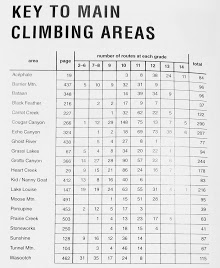
\includegraphics[width=0.4\textwidth]{key_climbing_areas.jpg}
  \caption{Chart showing distribution of climbing grades (diffuculty) at each crag in the \emph{Sport Climbs in the Canadian Rockies}}
  \label{fig:grade_distribution}
\end{figure}

\subsection{Crag Details and Route Selection}

All four books start the area sections with an overview page for the climbing area. This provides details on how to access the crag, a short description of the area, and possibly a map of the area for larger crags (fig \ref{fig:maps}). All of the books also contained an actual photograph of the different sections of rock, with superimposed lines showing the routes (fig \ref{fig:route_photo}). In \emph{Bow Valley Sport} the superimposed lines are color coded by difficulty (green, blue, black, red). Some of the books also showed hand-drawn illustrations of the routes, with more details such as bolt location, and route length in metres (fig \ref{fig:route_drawing}). \emph{Bow Valley Sport} also provides a written description of the route, as well as symbols indicating any specific ``styles'' (pumpy, reachy, technical footwork, etc) the route may be, and a checkbox to tick when the climb has been completed (fig \ref{fig:route_descriptions}). 

\begin{figure}[!htb]
  \centering
  \begin{subfigure}[b]{0.4\textwidth}
    \centering
    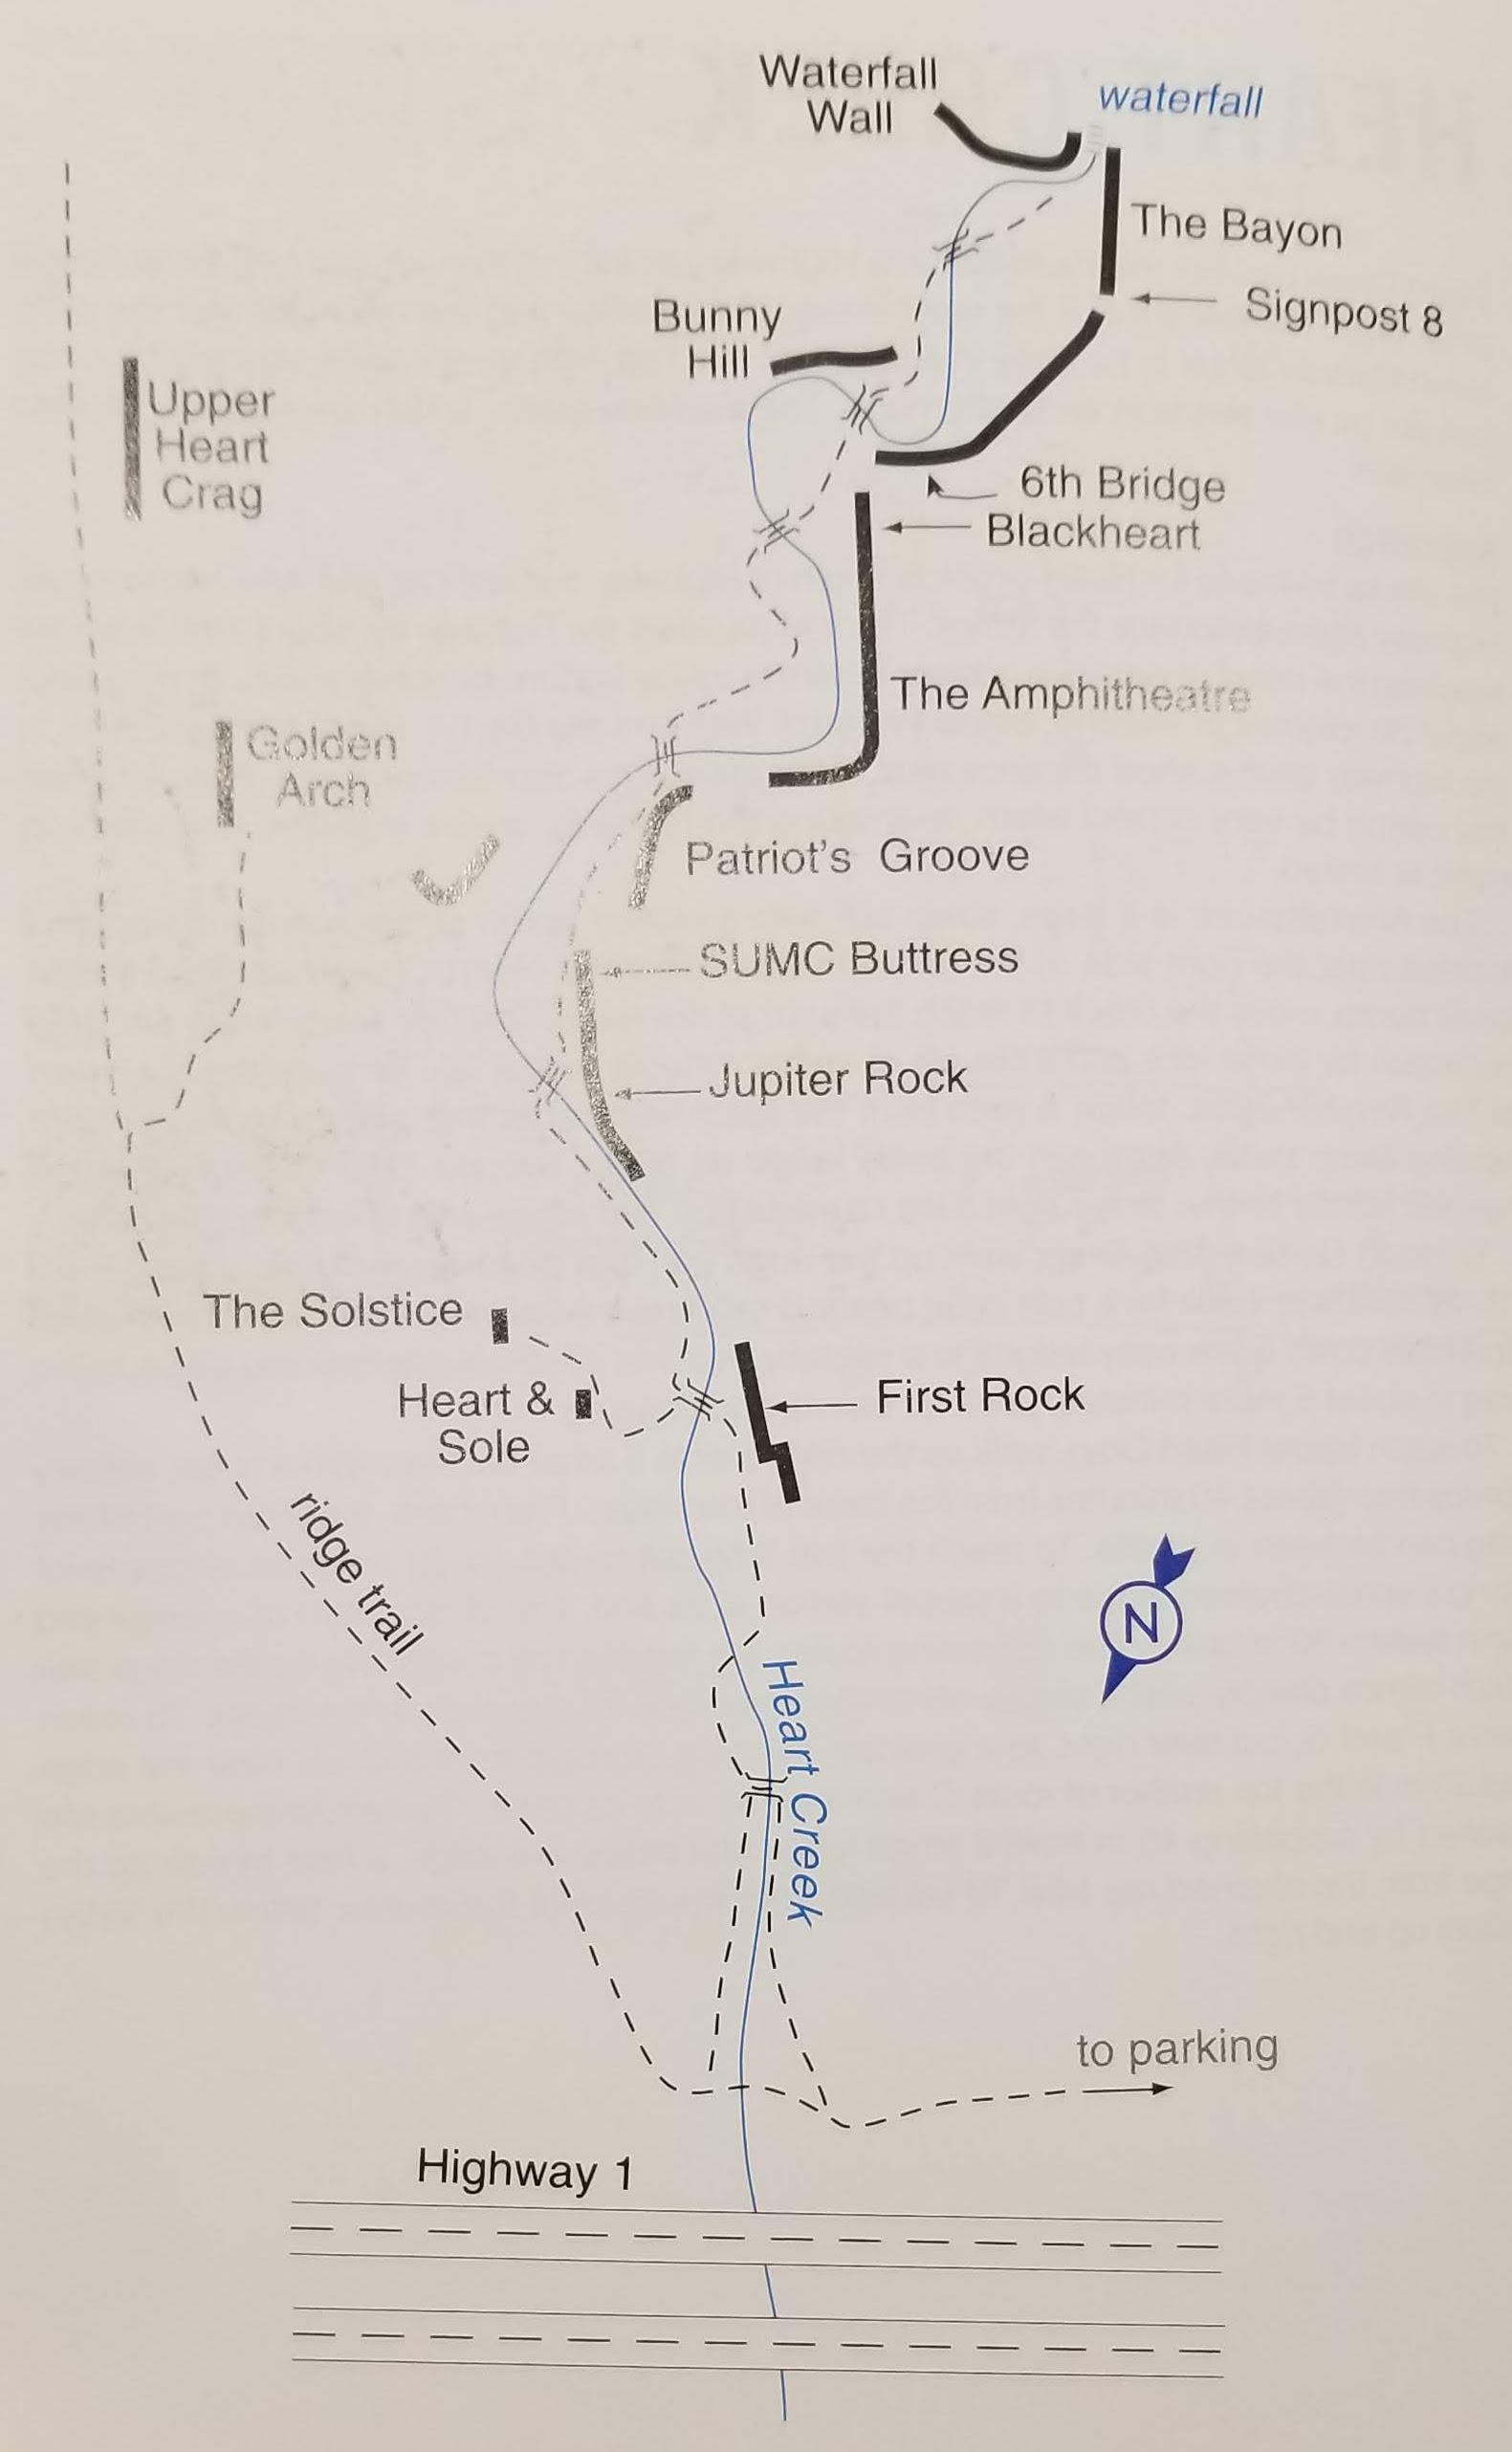
\includegraphics[height=\textwidth]{jupiter_rock_map_1.jpg}
    \caption{Sport Climbs in the Canadian Rockies}
\end{subfigure}
\begin{subfigure}[b]{0.4\textwidth}
    \centering
    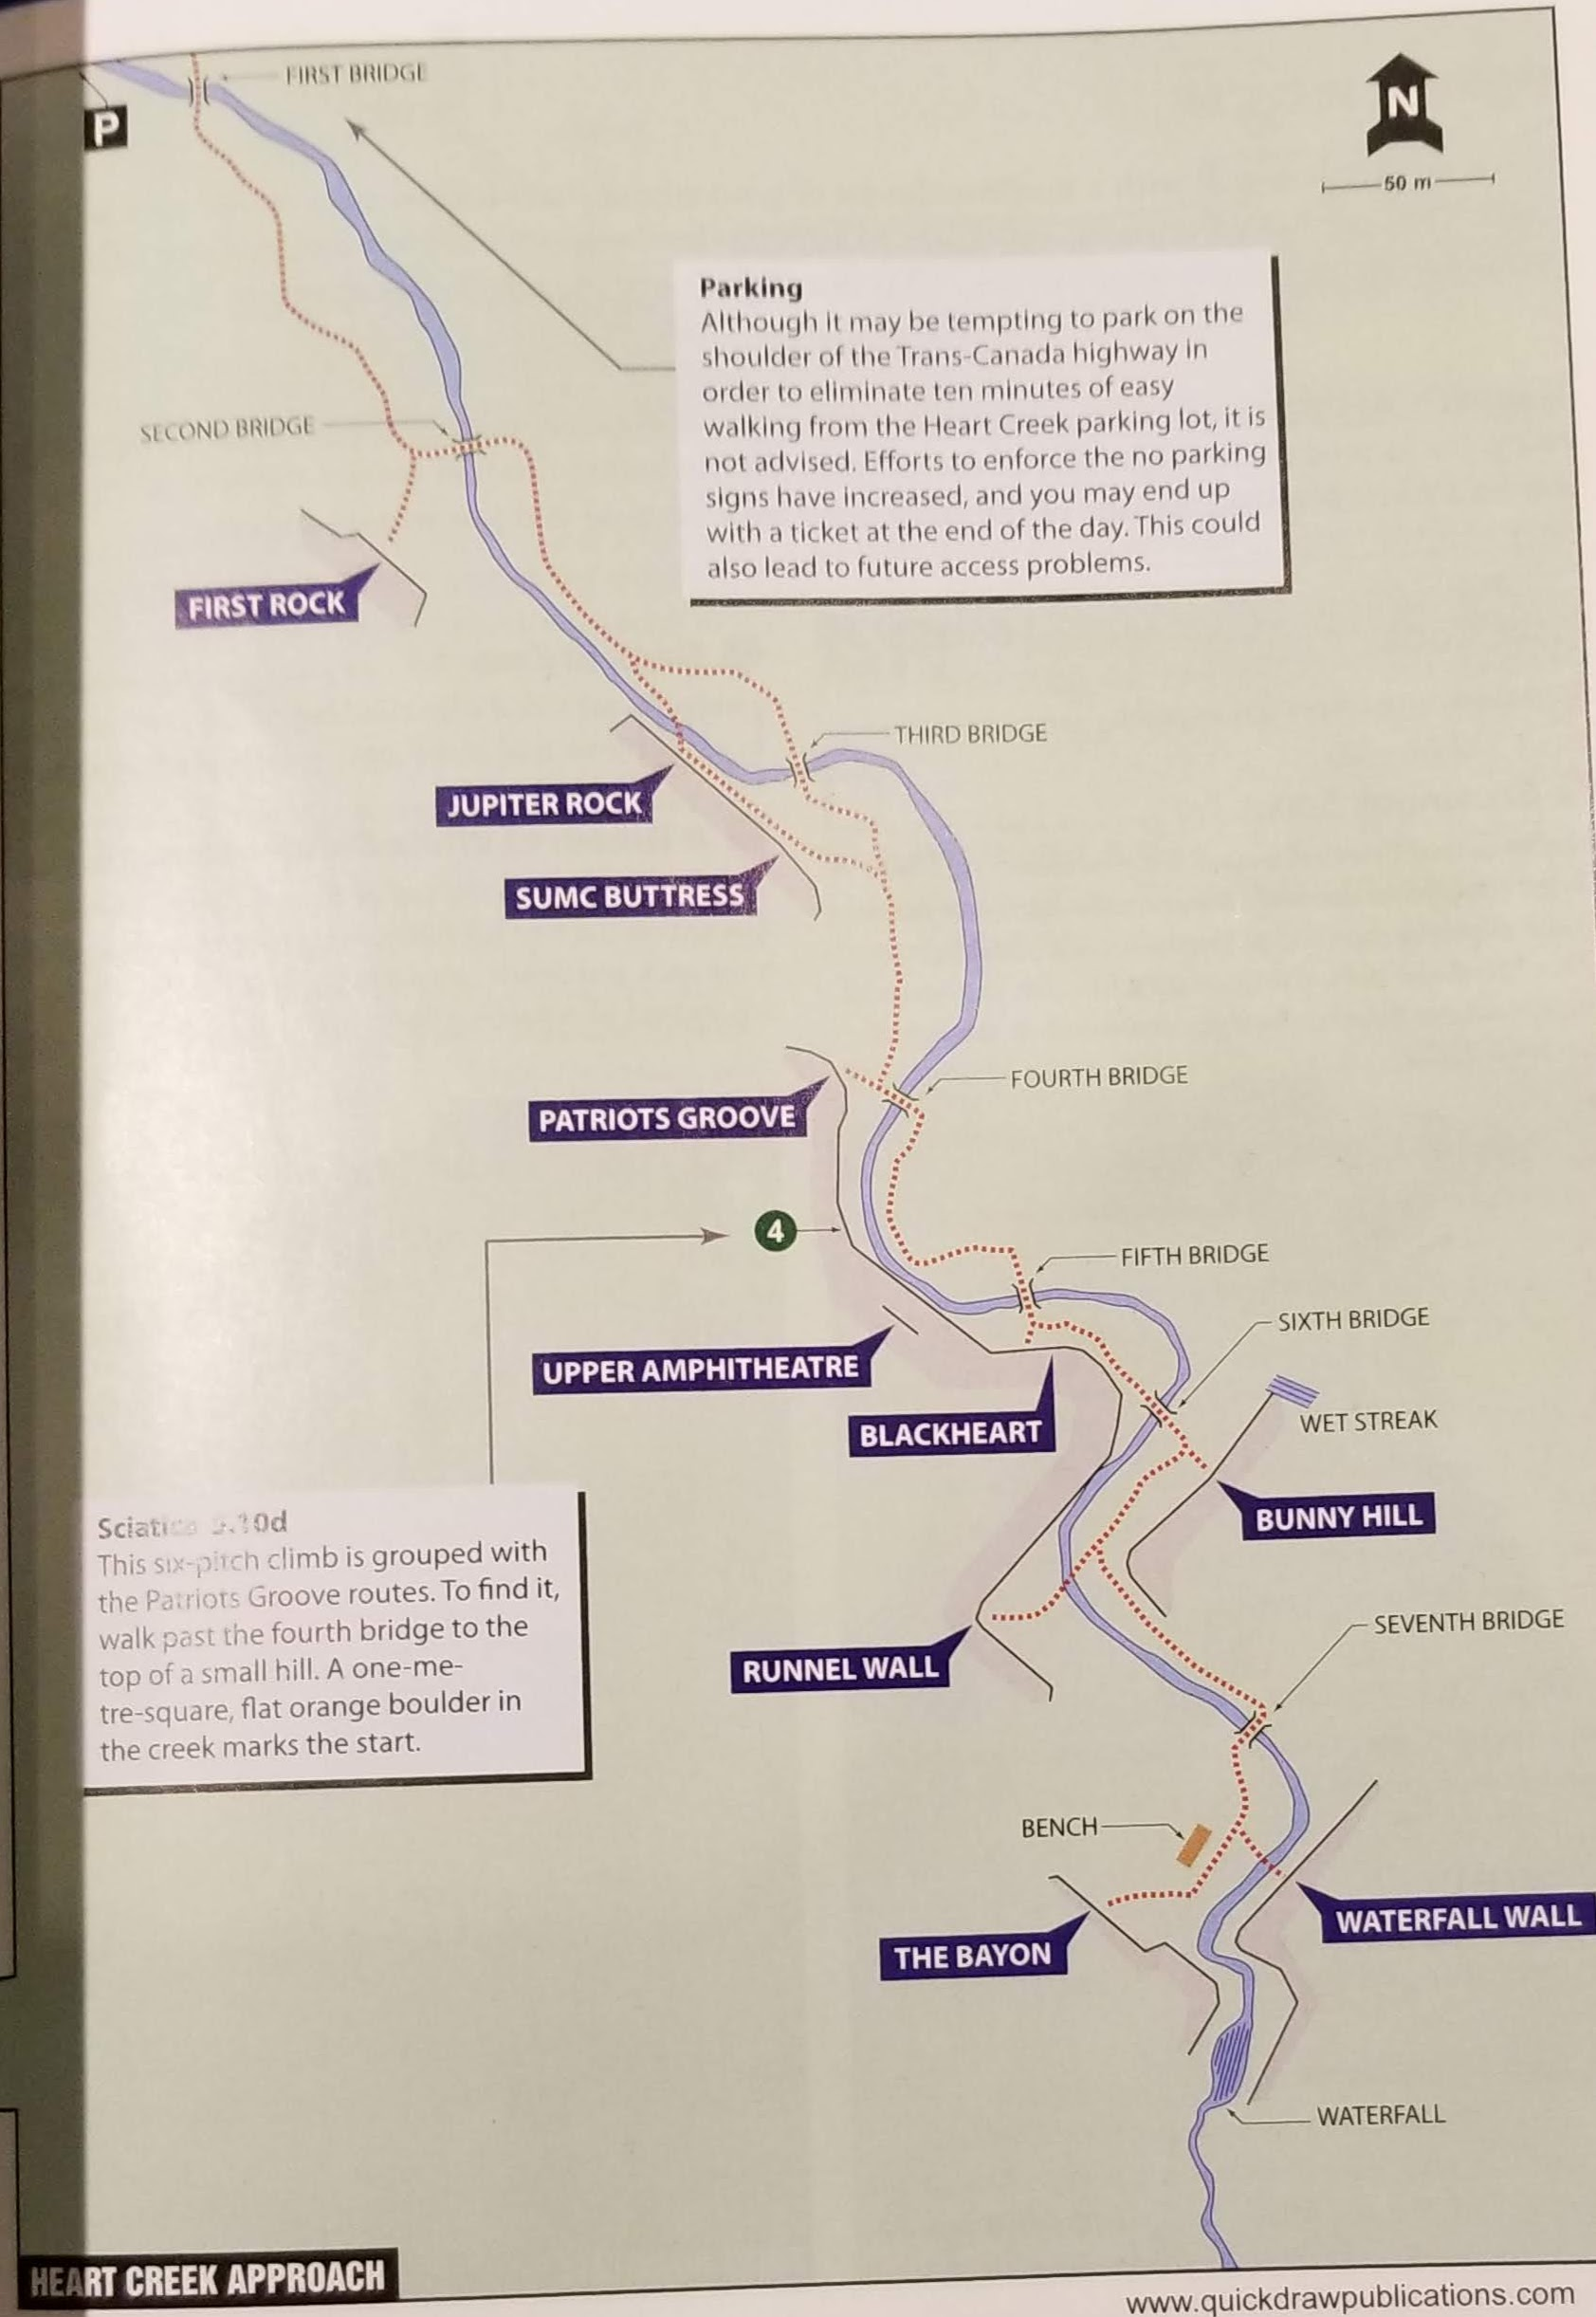
\includegraphics[height=\textwidth]{jupiter_rock_map_2.jpg}
    \caption{Bow Valley Sport}
\end{subfigure}
  \caption{Climbing area overview maps.}
  \label{fig:maps}
\end{figure}

\begin{figure}[!htb]
  \centering
  \begin{subfigure}[b]{0.3\textwidth}
    \centering
    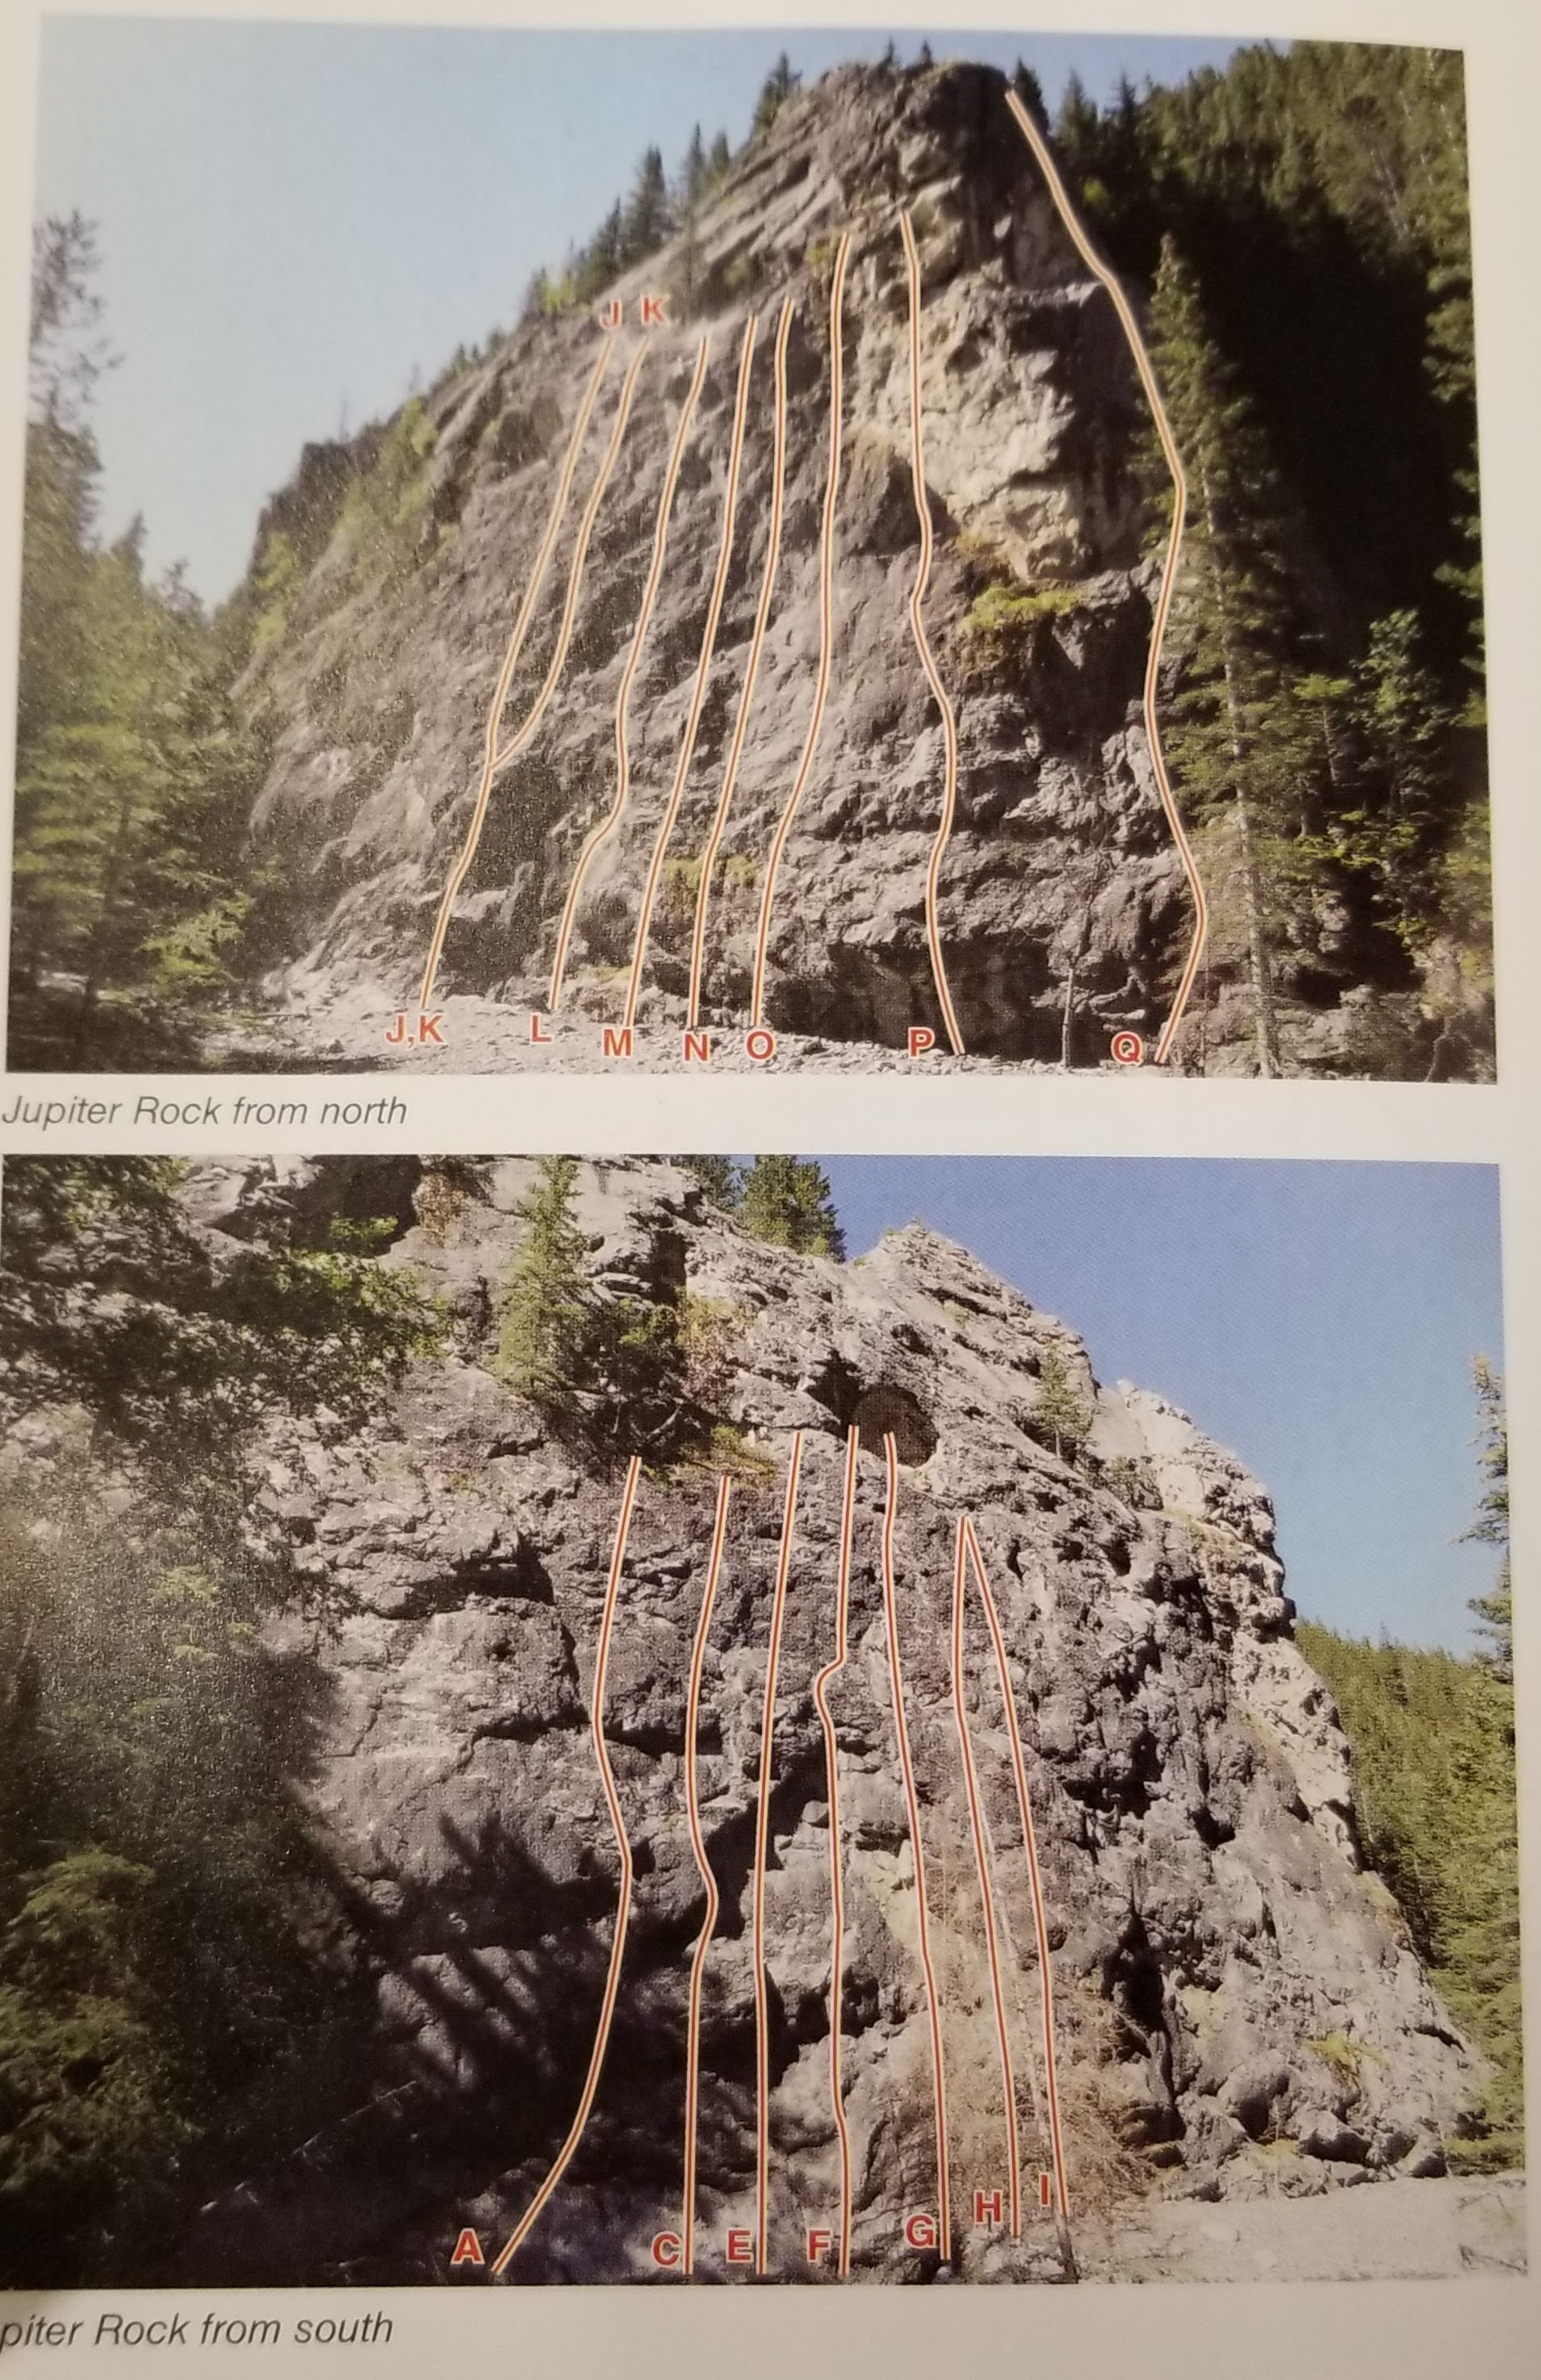
\includegraphics[width=\textwidth]{juptier_rock_photo.jpg}
    \caption{Photograph of rock with superimposed routes.}
    \label{fig:route_photo}
  \end{subfigure}
  \hfill
  \begin{subfigure}[b]{0.3\textwidth}
    \centering
    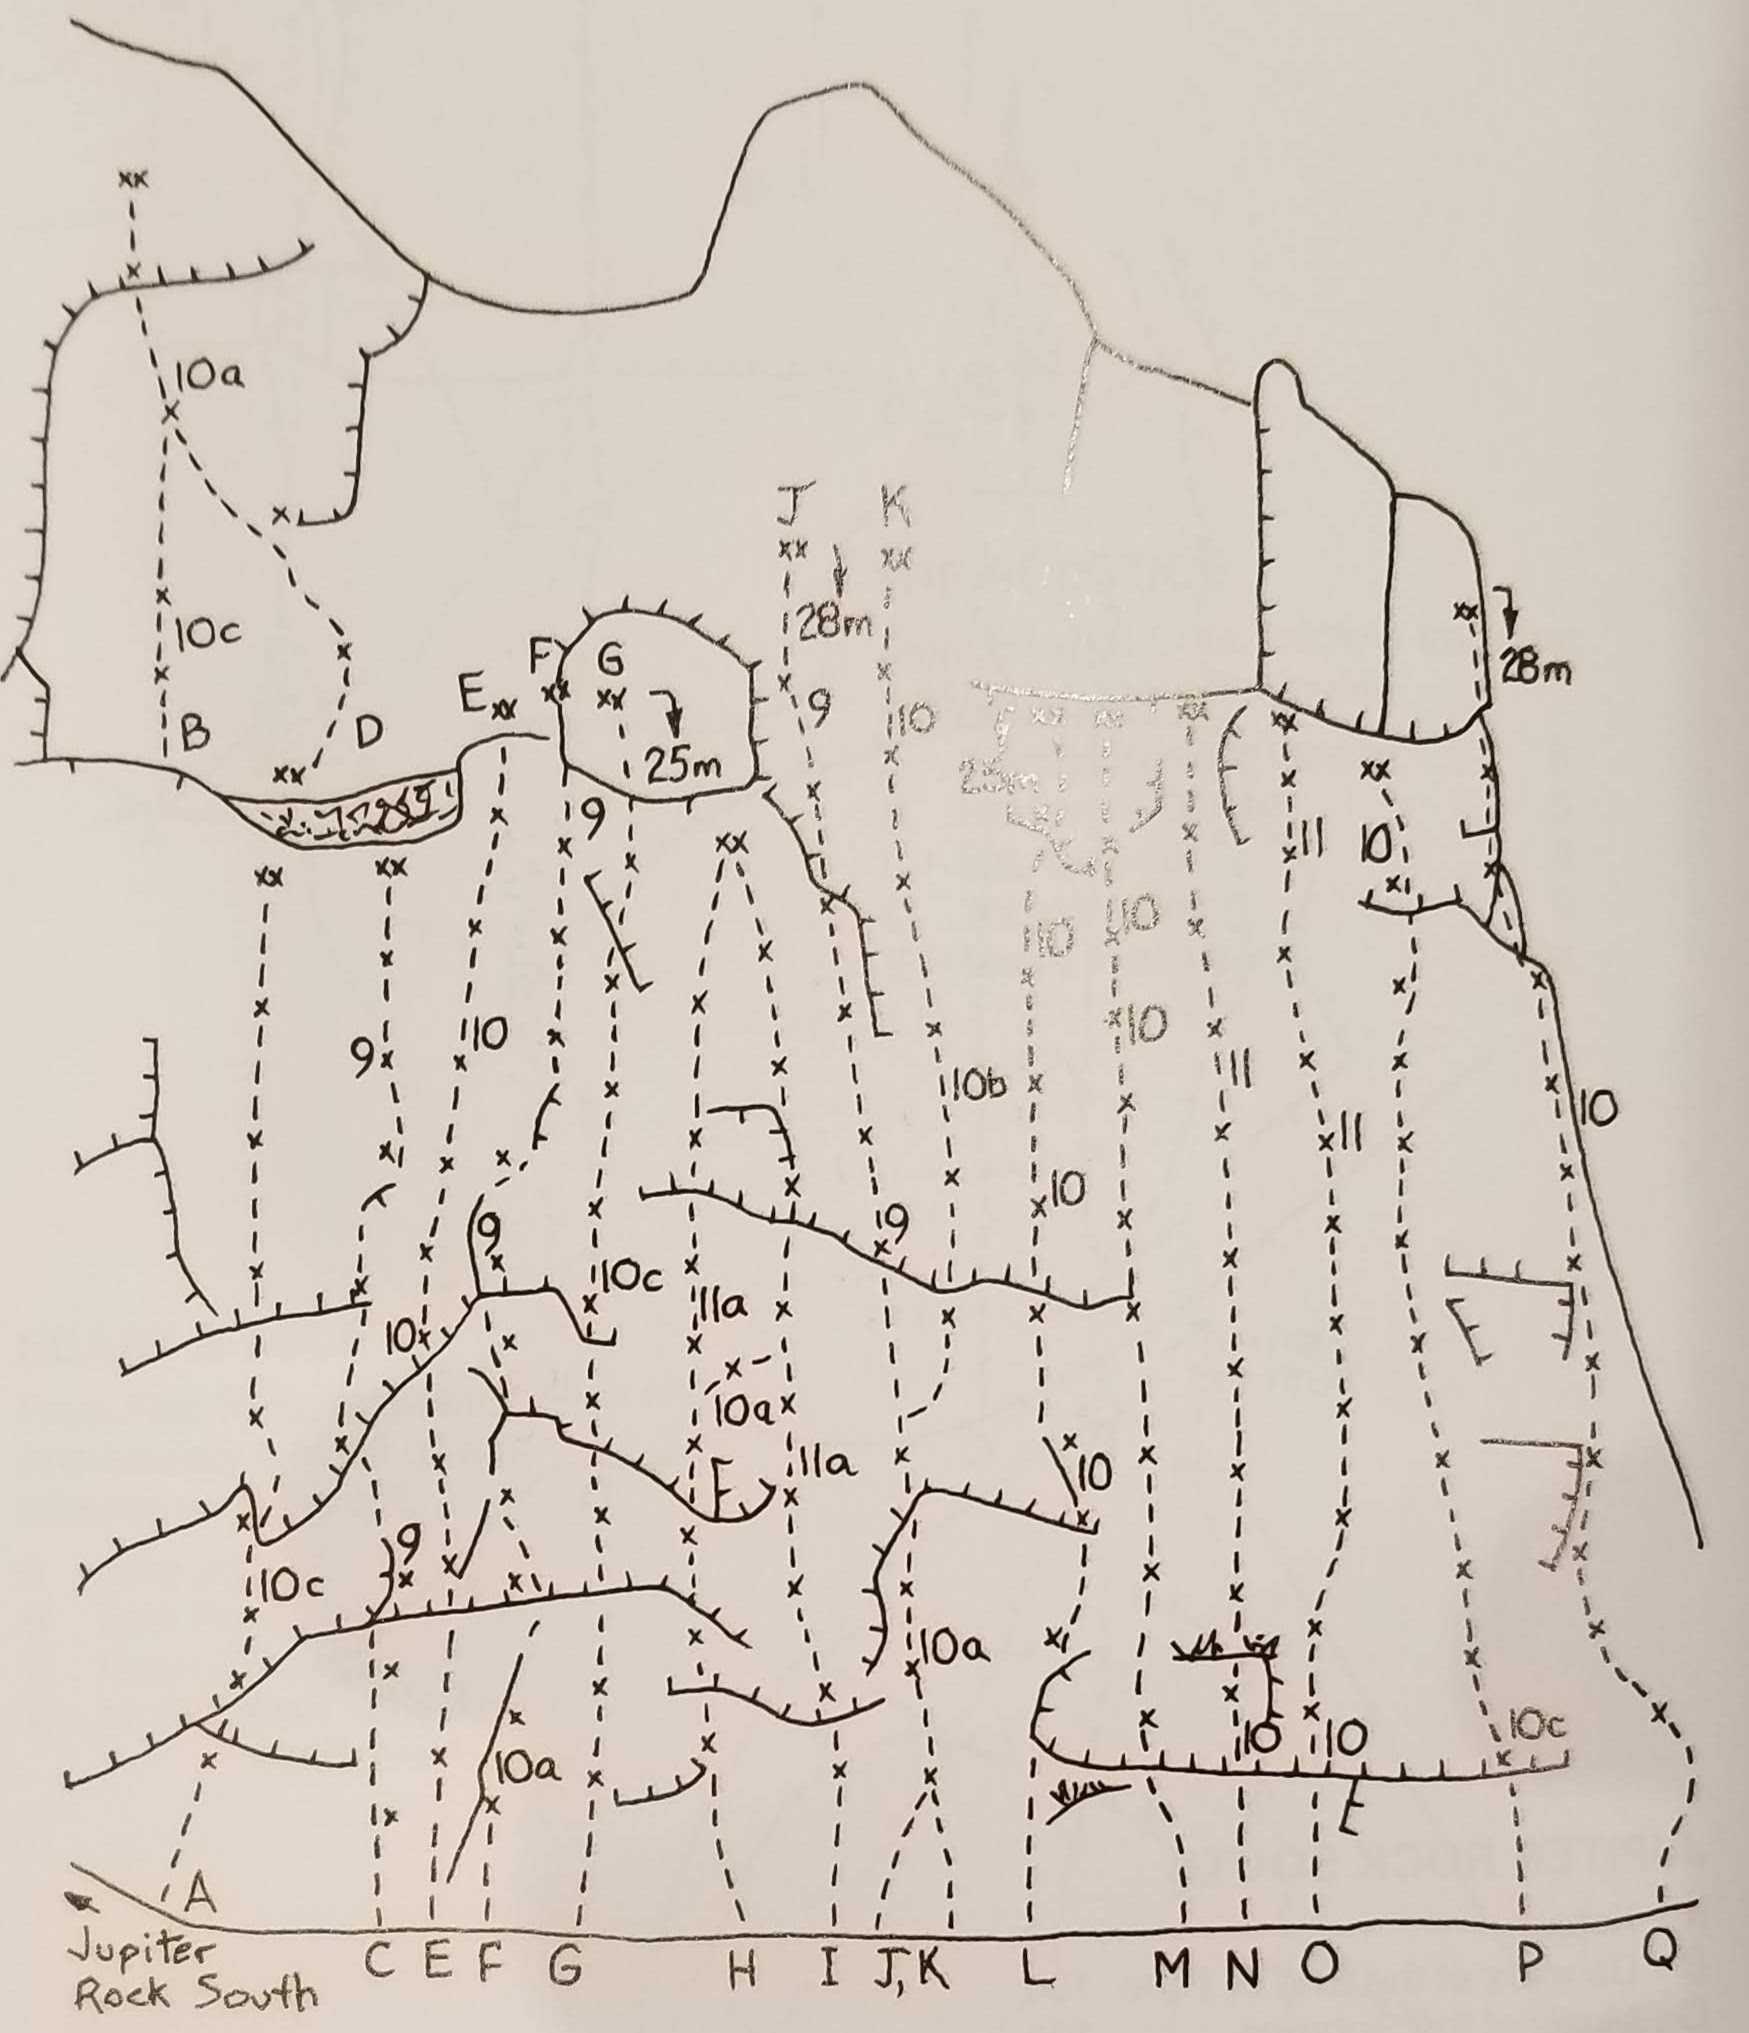
\includegraphics[width=\textwidth]{jupiter_rock_drawing.jpg}
    \caption{Drawing of routes on rock with bolt locations and height above ground.}
    \label{fig:route_drawing}
  \end{subfigure}
  \hfill
  \begin{subfigure}[b]{0.3\textwidth}
    \centering
    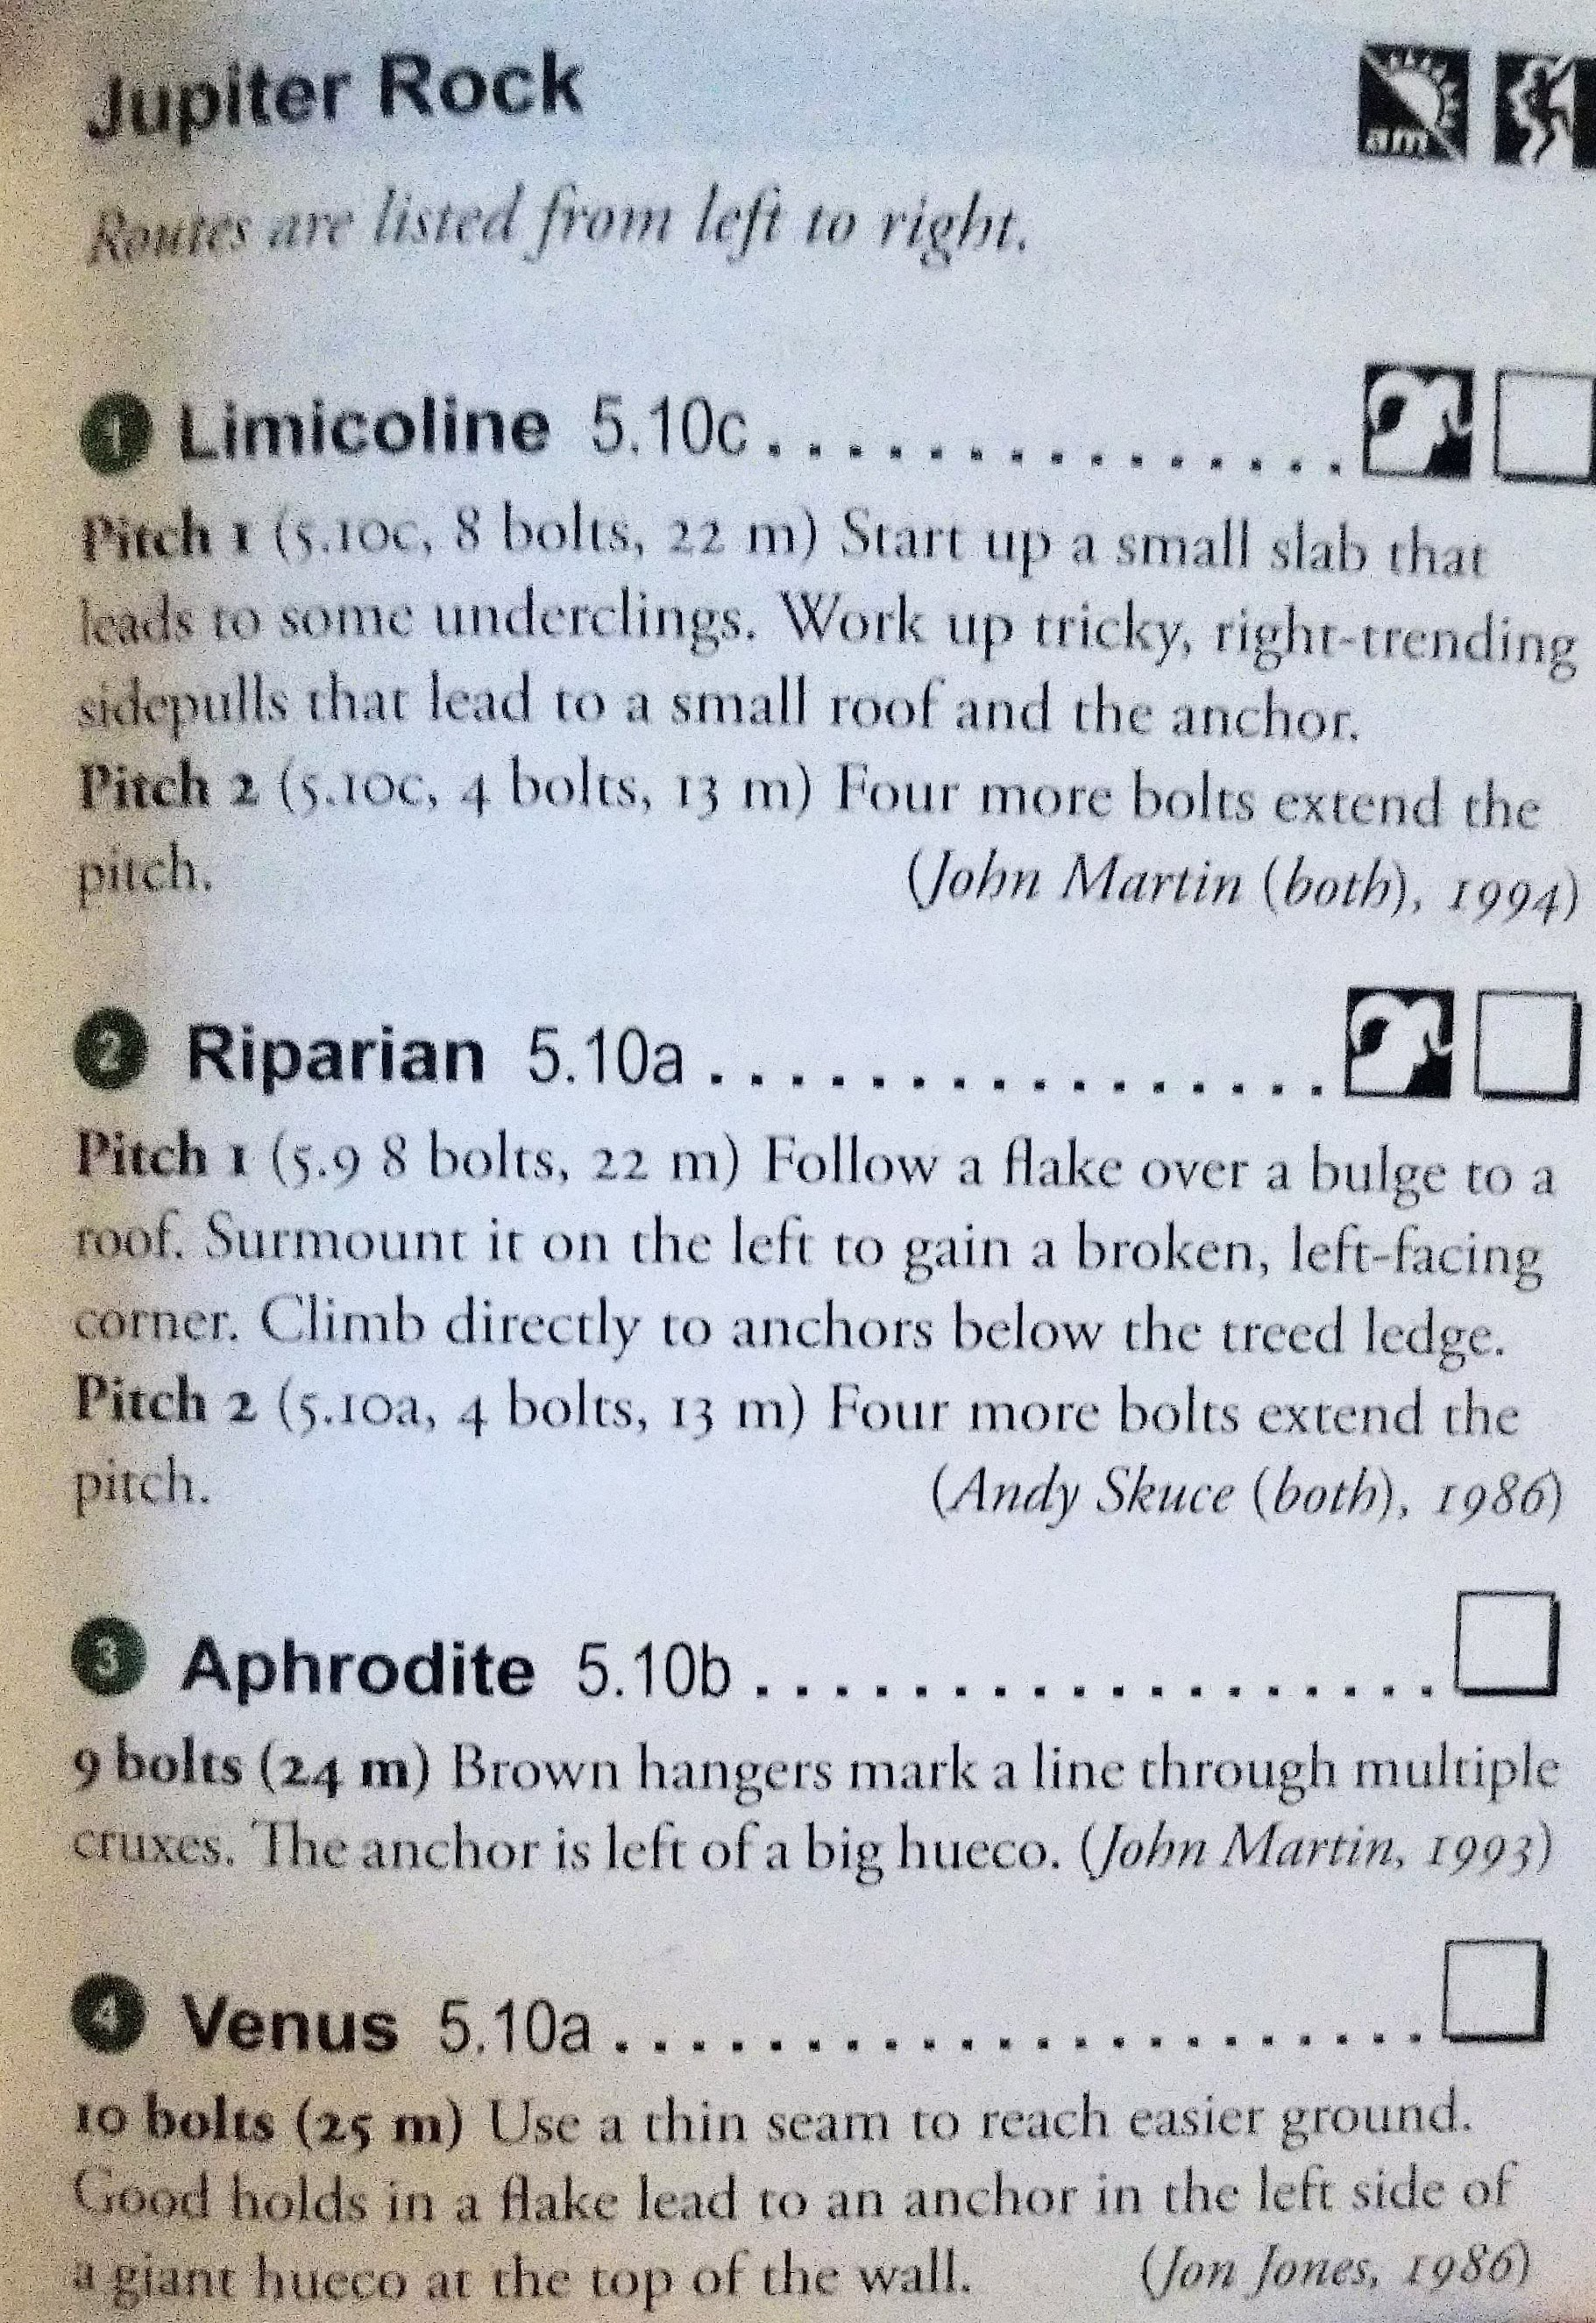
\includegraphics[width=\textwidth]{jupiter_rock_descriptions.jpg}
    \caption{Detailed Route Descriptions and Style}
    \label{fig:route_descriptions}
  \end{subfigure}
  \caption{Route location and descriptions from the guidebooks.}
\end{figure}

\section{Mobile Applications}

\emph{The Mountain Project} is a mobile application somewhat similar to the product we intend to design. The main interface (fig \ref{fig:mp_main}) contains buttons to find routes/areas near the user, to search by name, or to view routes on a todo-list. To find a specific climbing area, the user first searches by name, taps on the area, and is then taken to to the area overview screen (fig \ref{fig:area_overview}).

\begin{figure}[!htb]
  \centering
  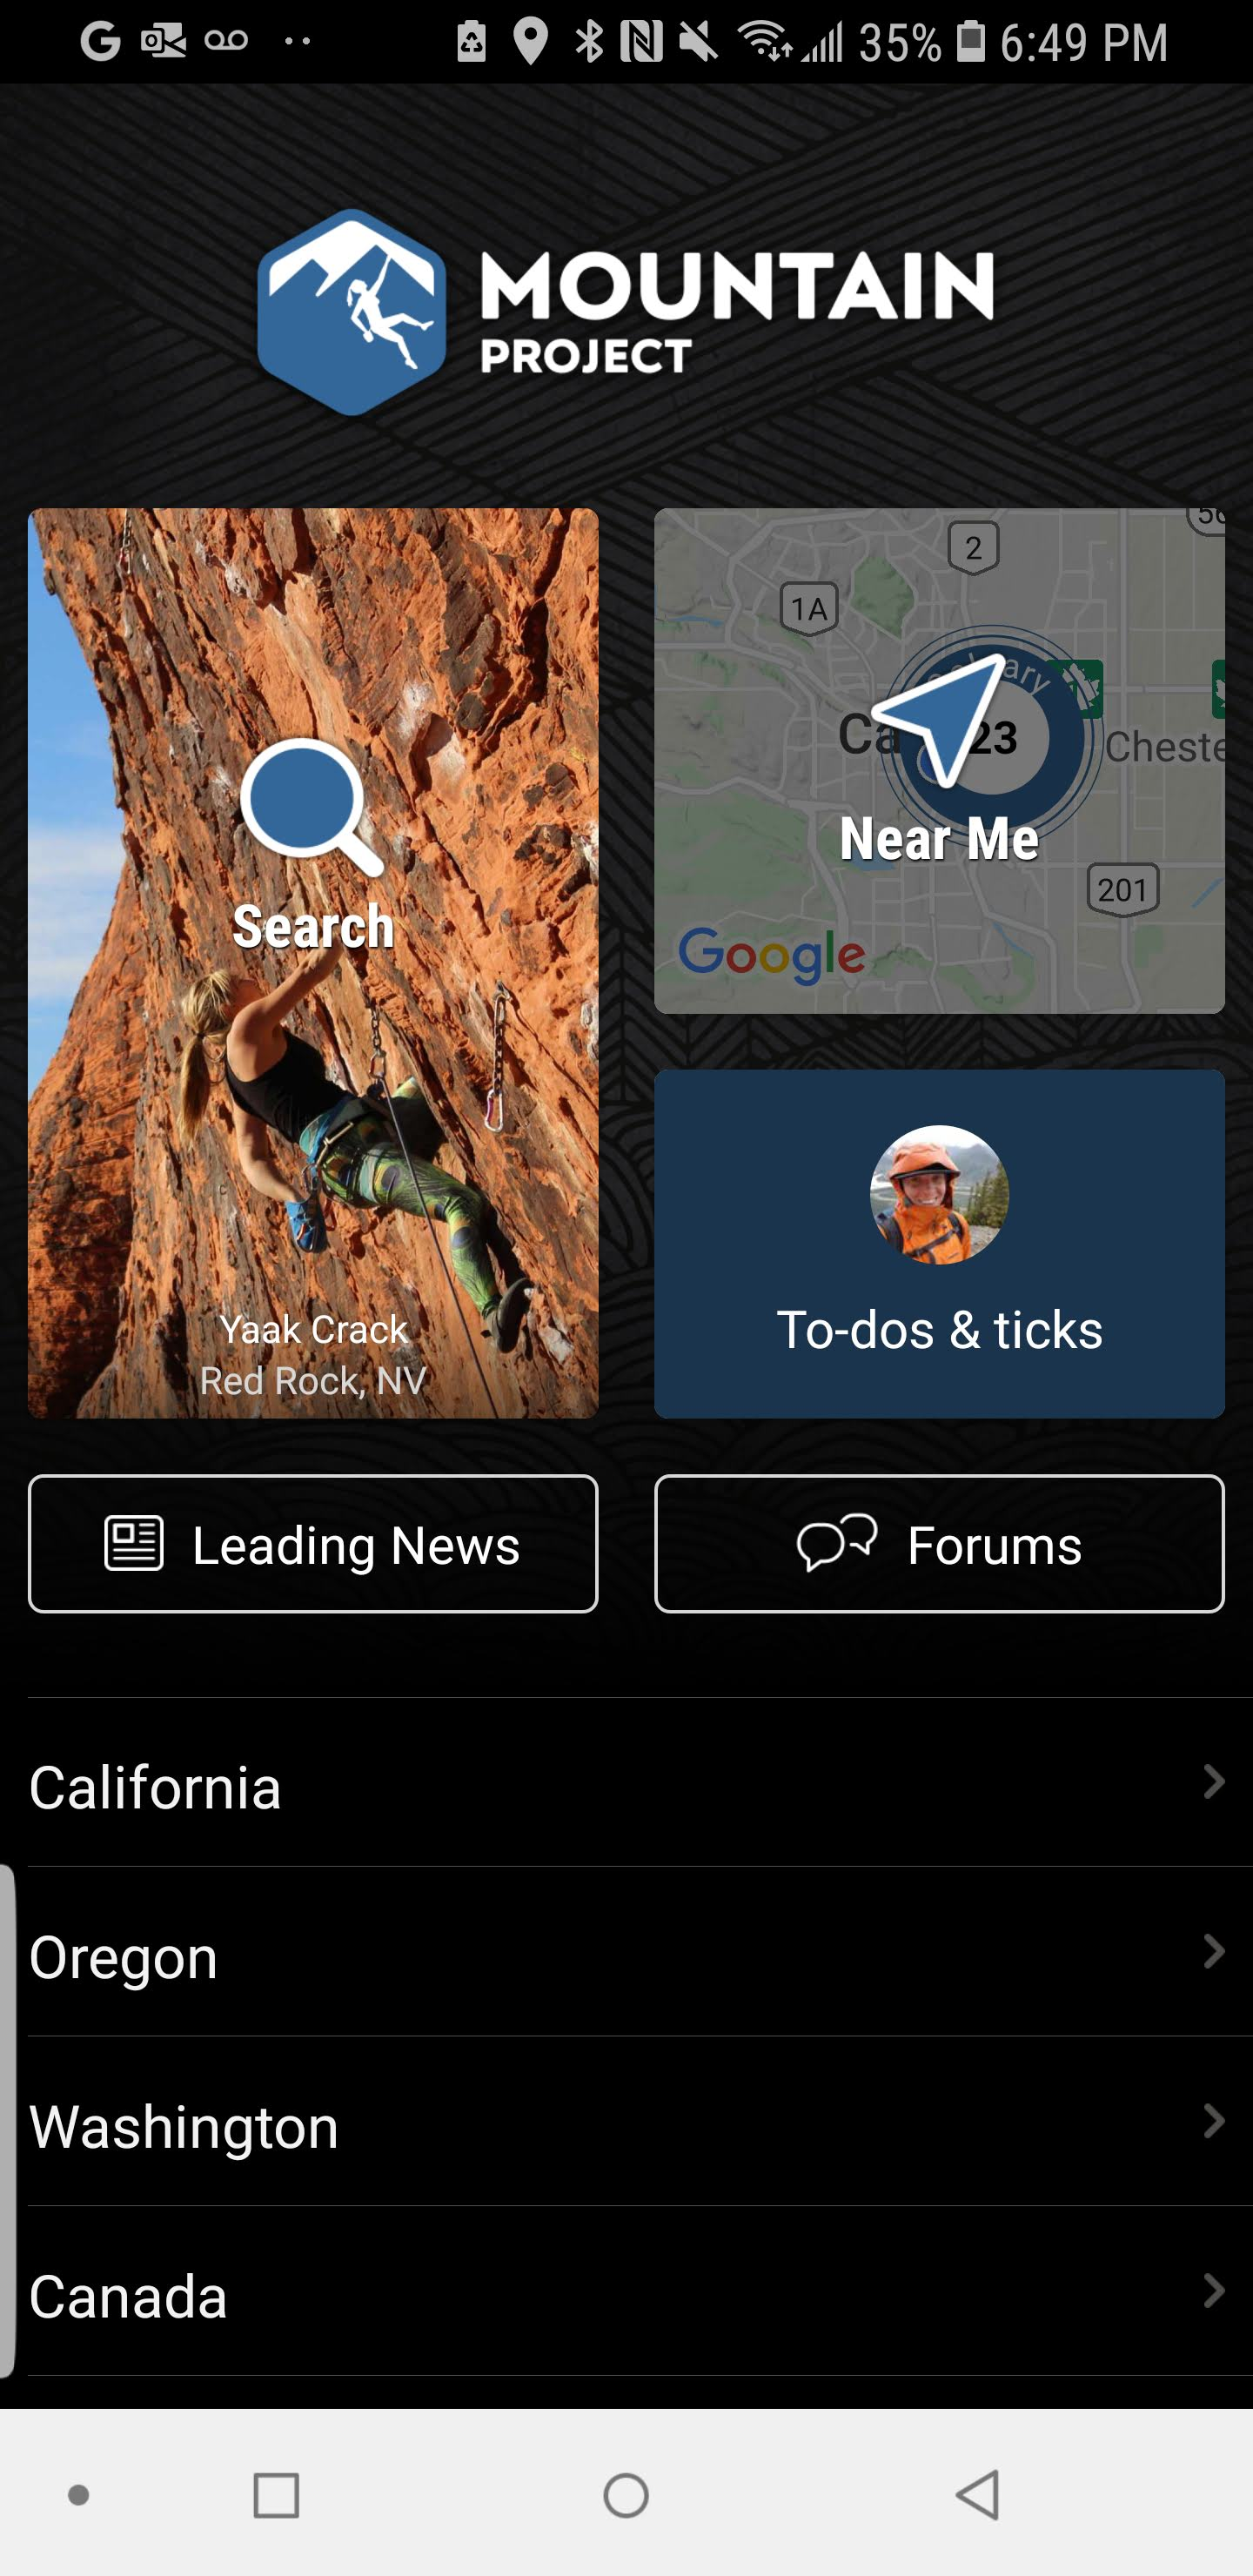
\includegraphics[width=0.25\textwidth]{mp_home.jpg}
  \caption{Main screen of \emph{The Mountain Project} application.}
  \label{fig:mp_main}
\end{figure}

Much like in the guidebooks, the climbing areas are further divided into the (named) rock faces. The routes are displayed in a list format (fig \ref{fig:face_list}). Again, tapping on a named rock face shows an overview of the face (fig \ref{fig:face_overview}). Tapping on a route displays information about the route, and possible a photograph of it. There is also functionality for users to add the route to their todo list, tick it when done, rate the climb, and share (fig \ref{fig:mp_callisto}).

\begin{figure}[!h]
  \centering
  \begin{subfigure}[b]{0.3\textwidth}
      \centering
      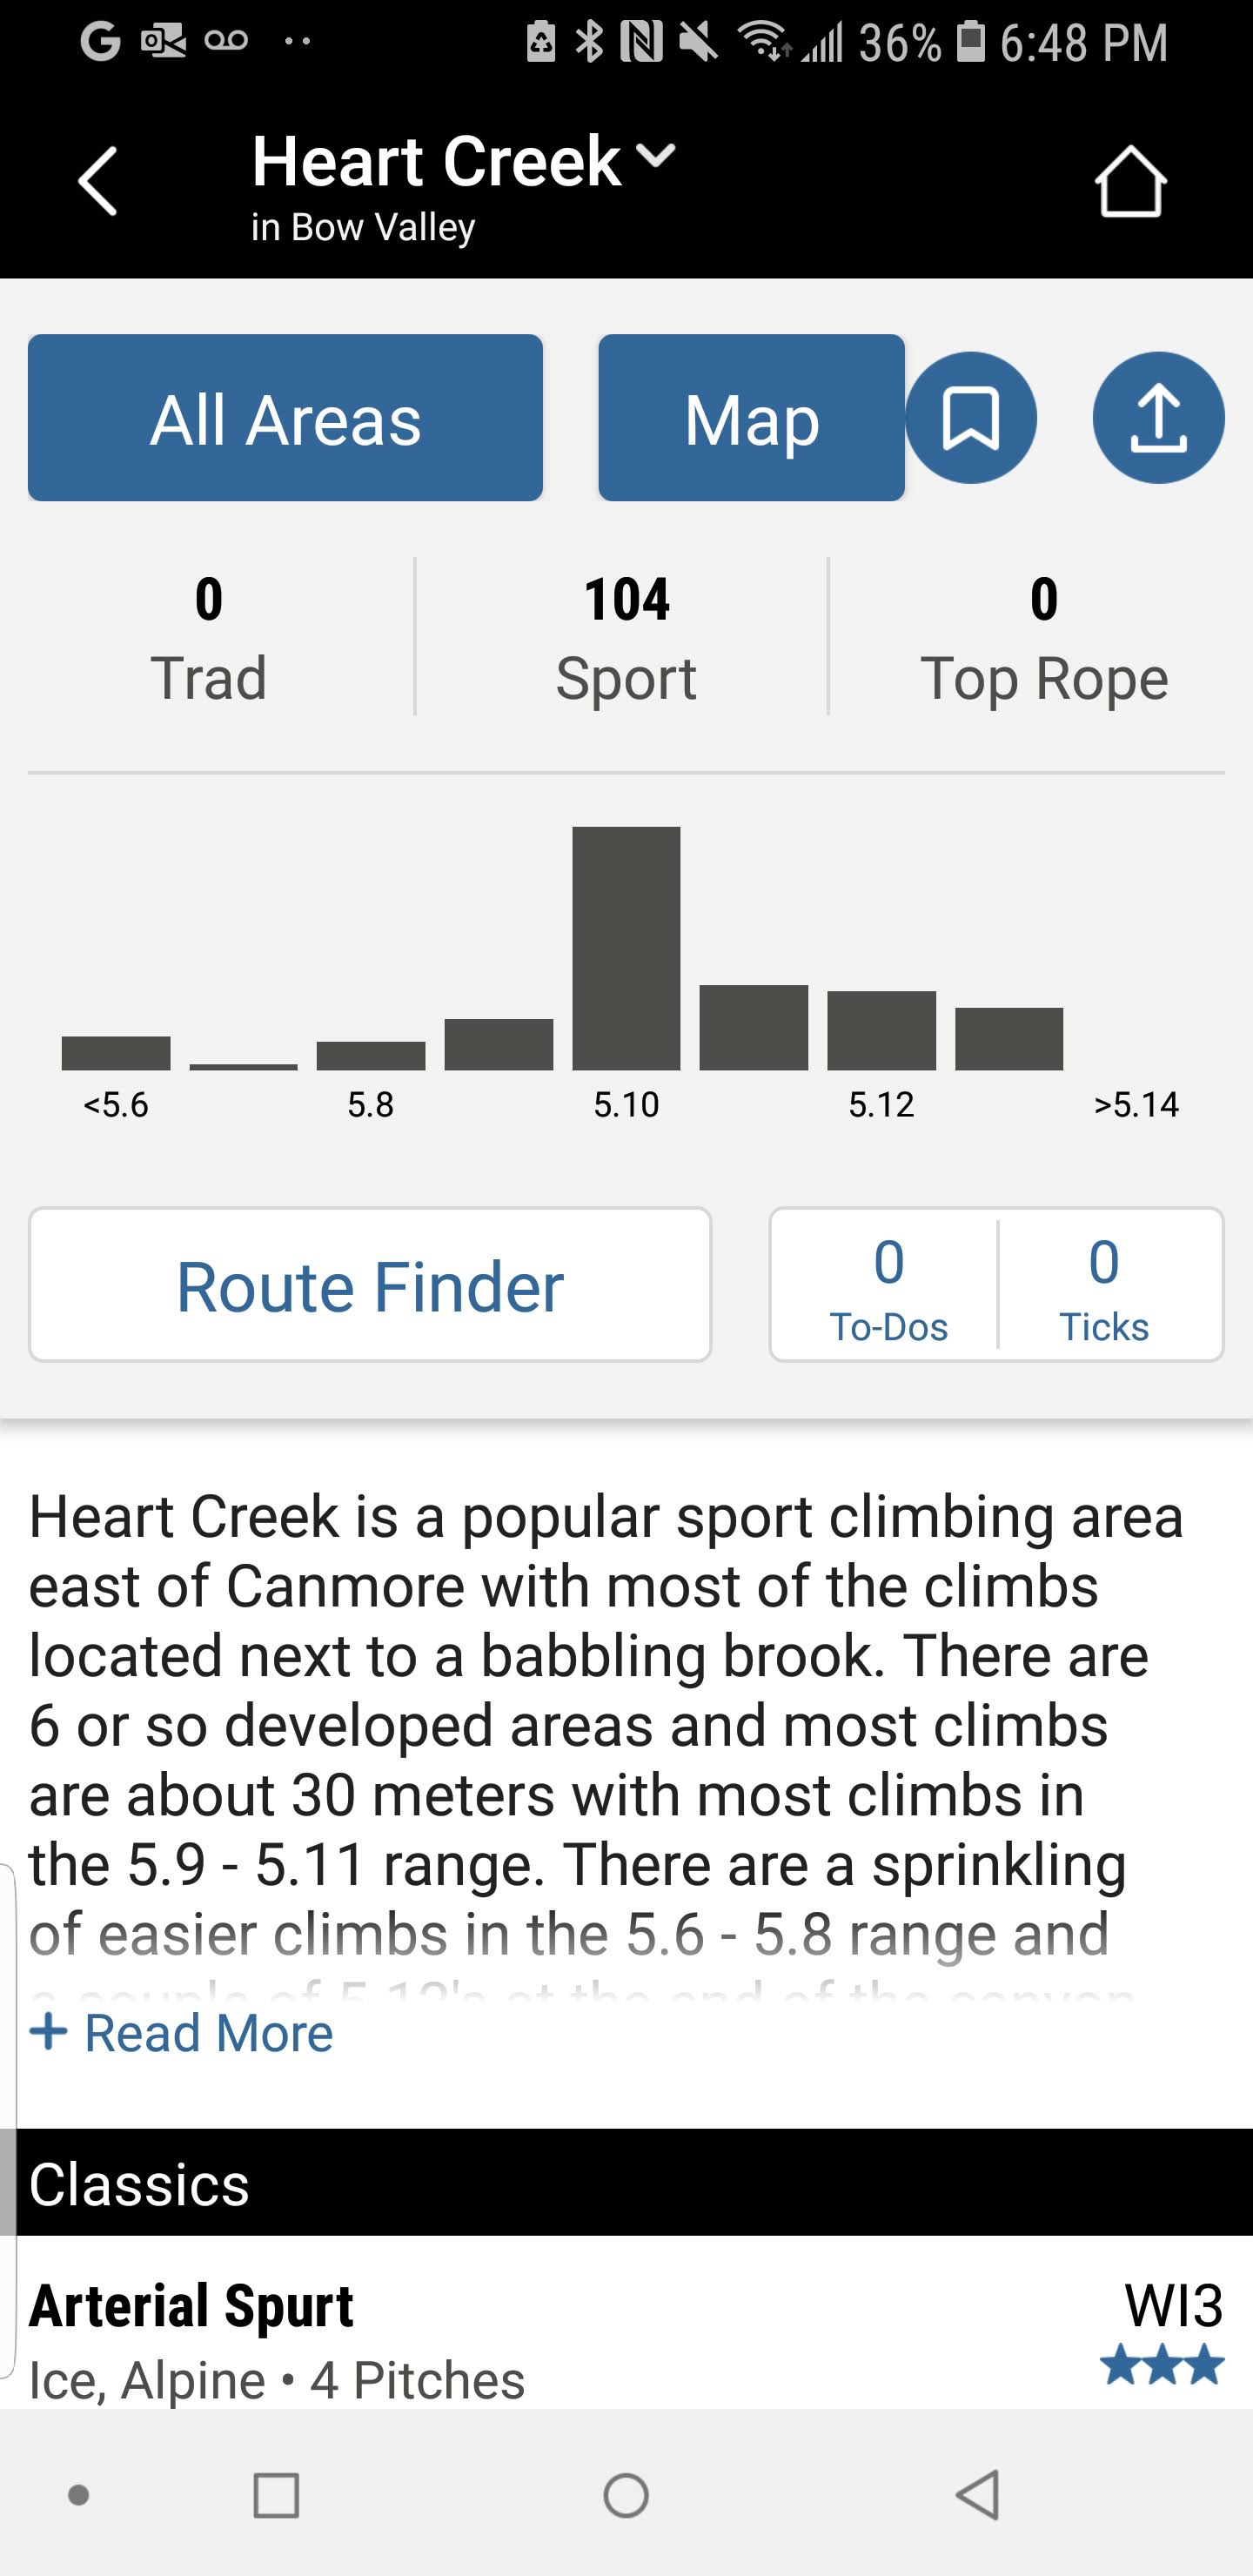
\includegraphics[width=\textwidth]{mp_heart_creek.jpg}
      \caption{Area Overview}
      \label{fig:area_overview}
  \end{subfigure}
  \hfill
  \begin{subfigure}[b]{0.3\textwidth}
      \centering
      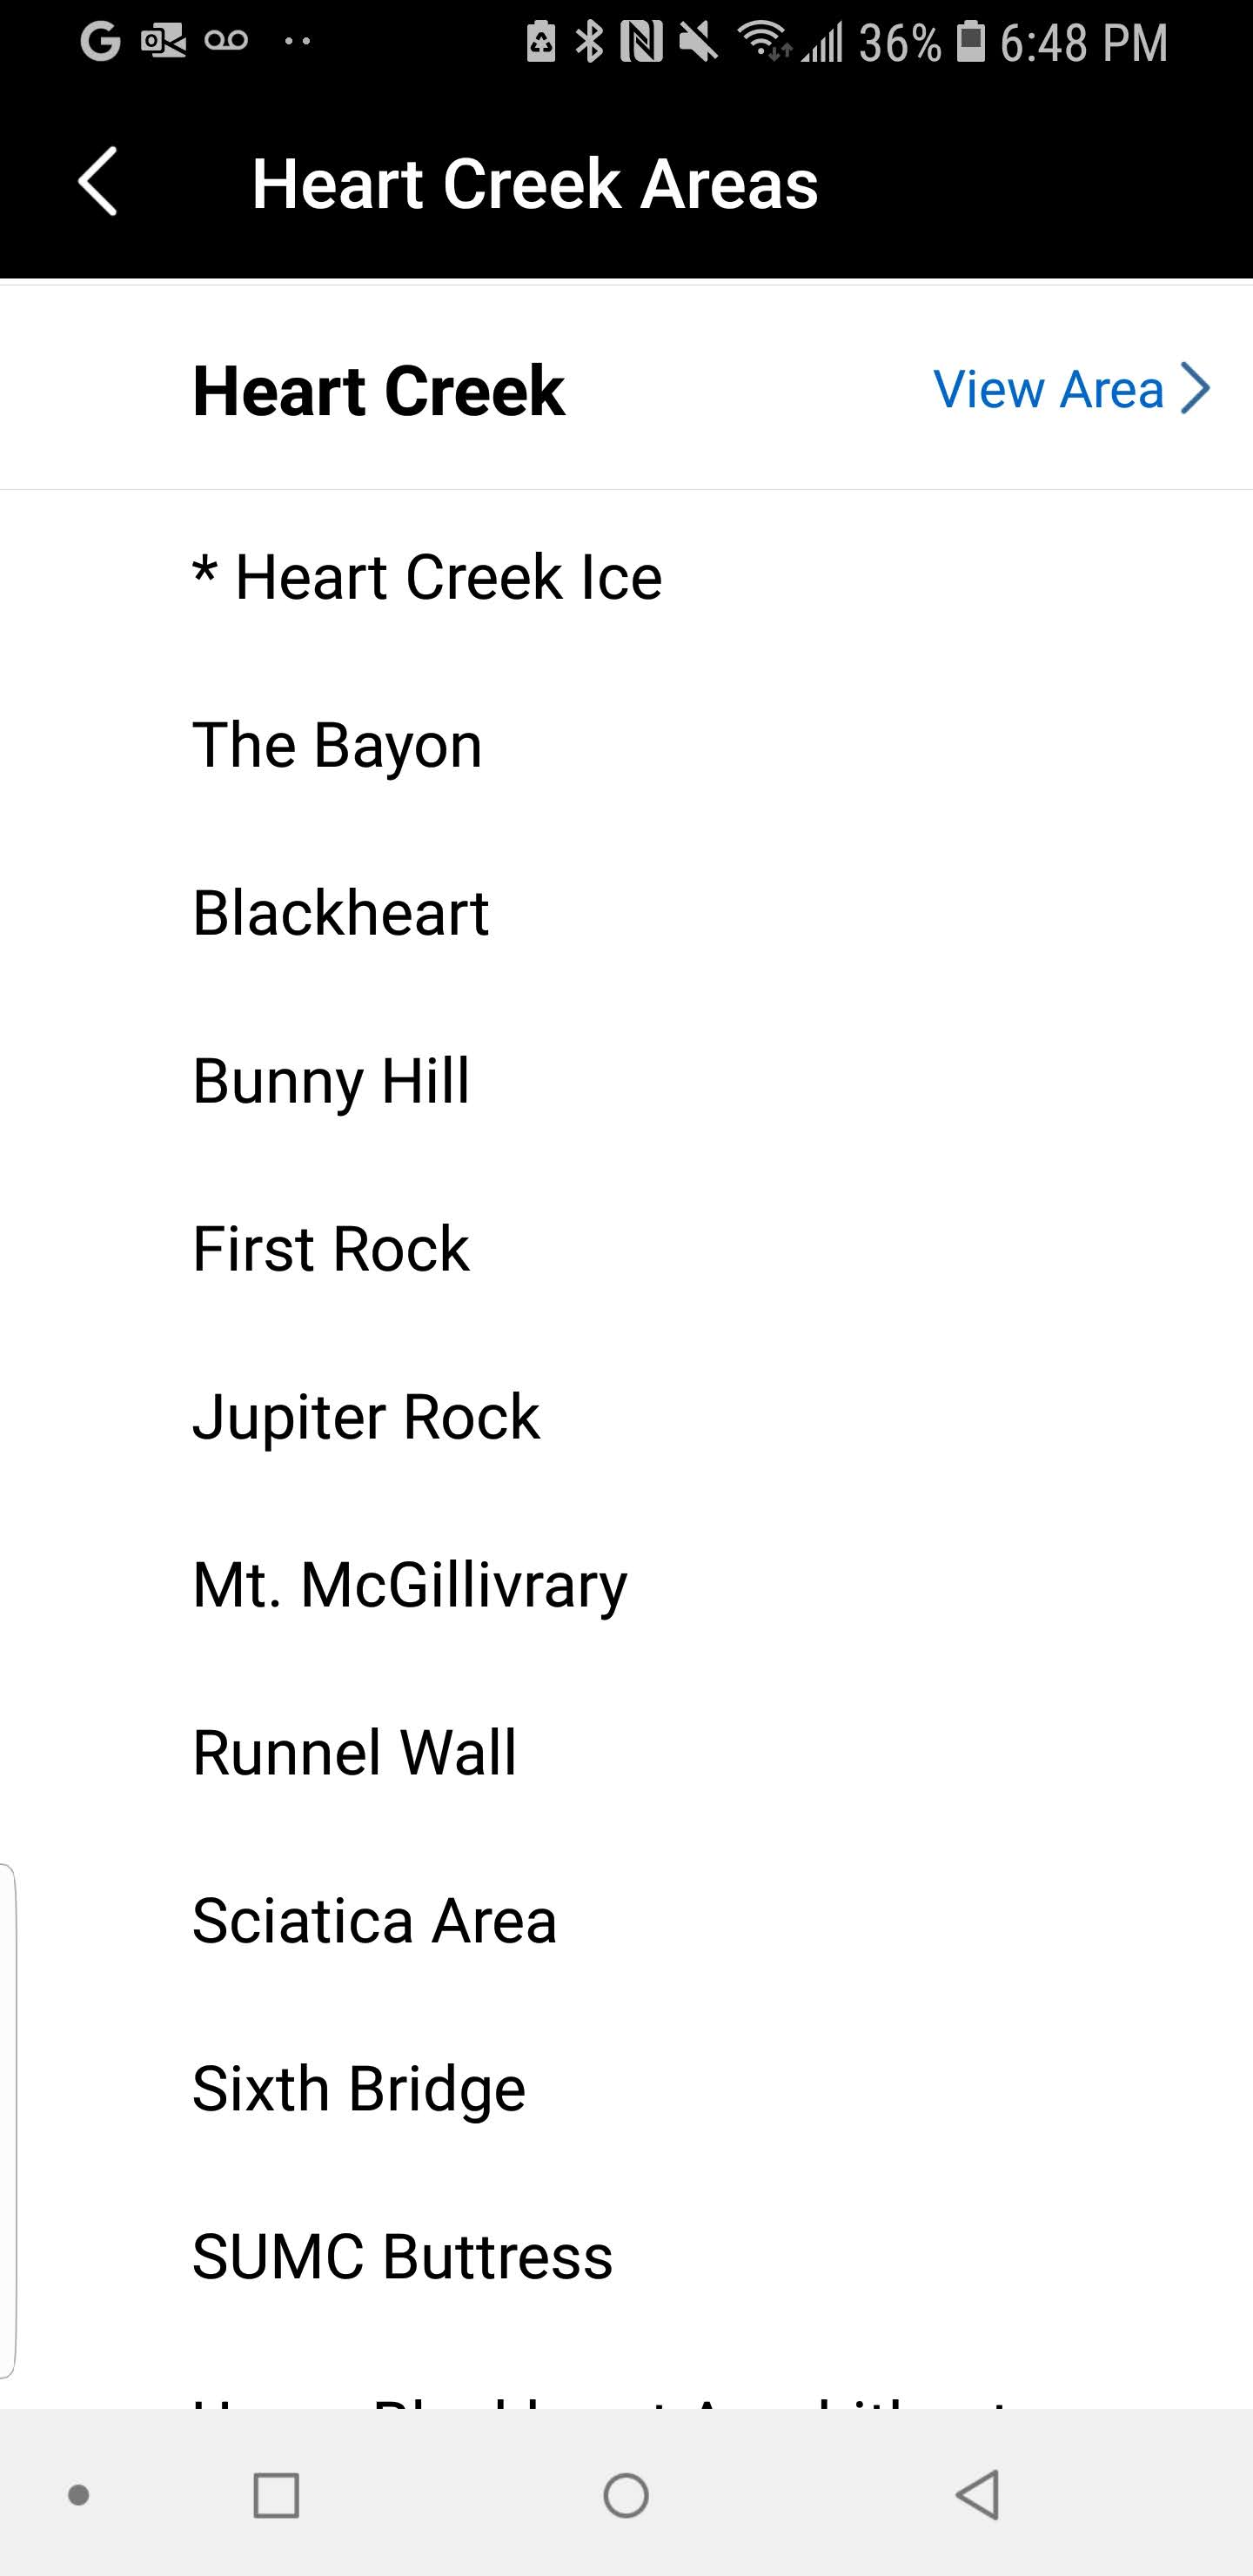
\includegraphics[width=\textwidth]{mp_hear_creek_toc.jpg}
      \caption{Rock faces in the area}
      \label{fig:face_list}
  \end{subfigure}
  \hfill
  \begin{subfigure}[b]{0.3\textwidth}
      \centering
      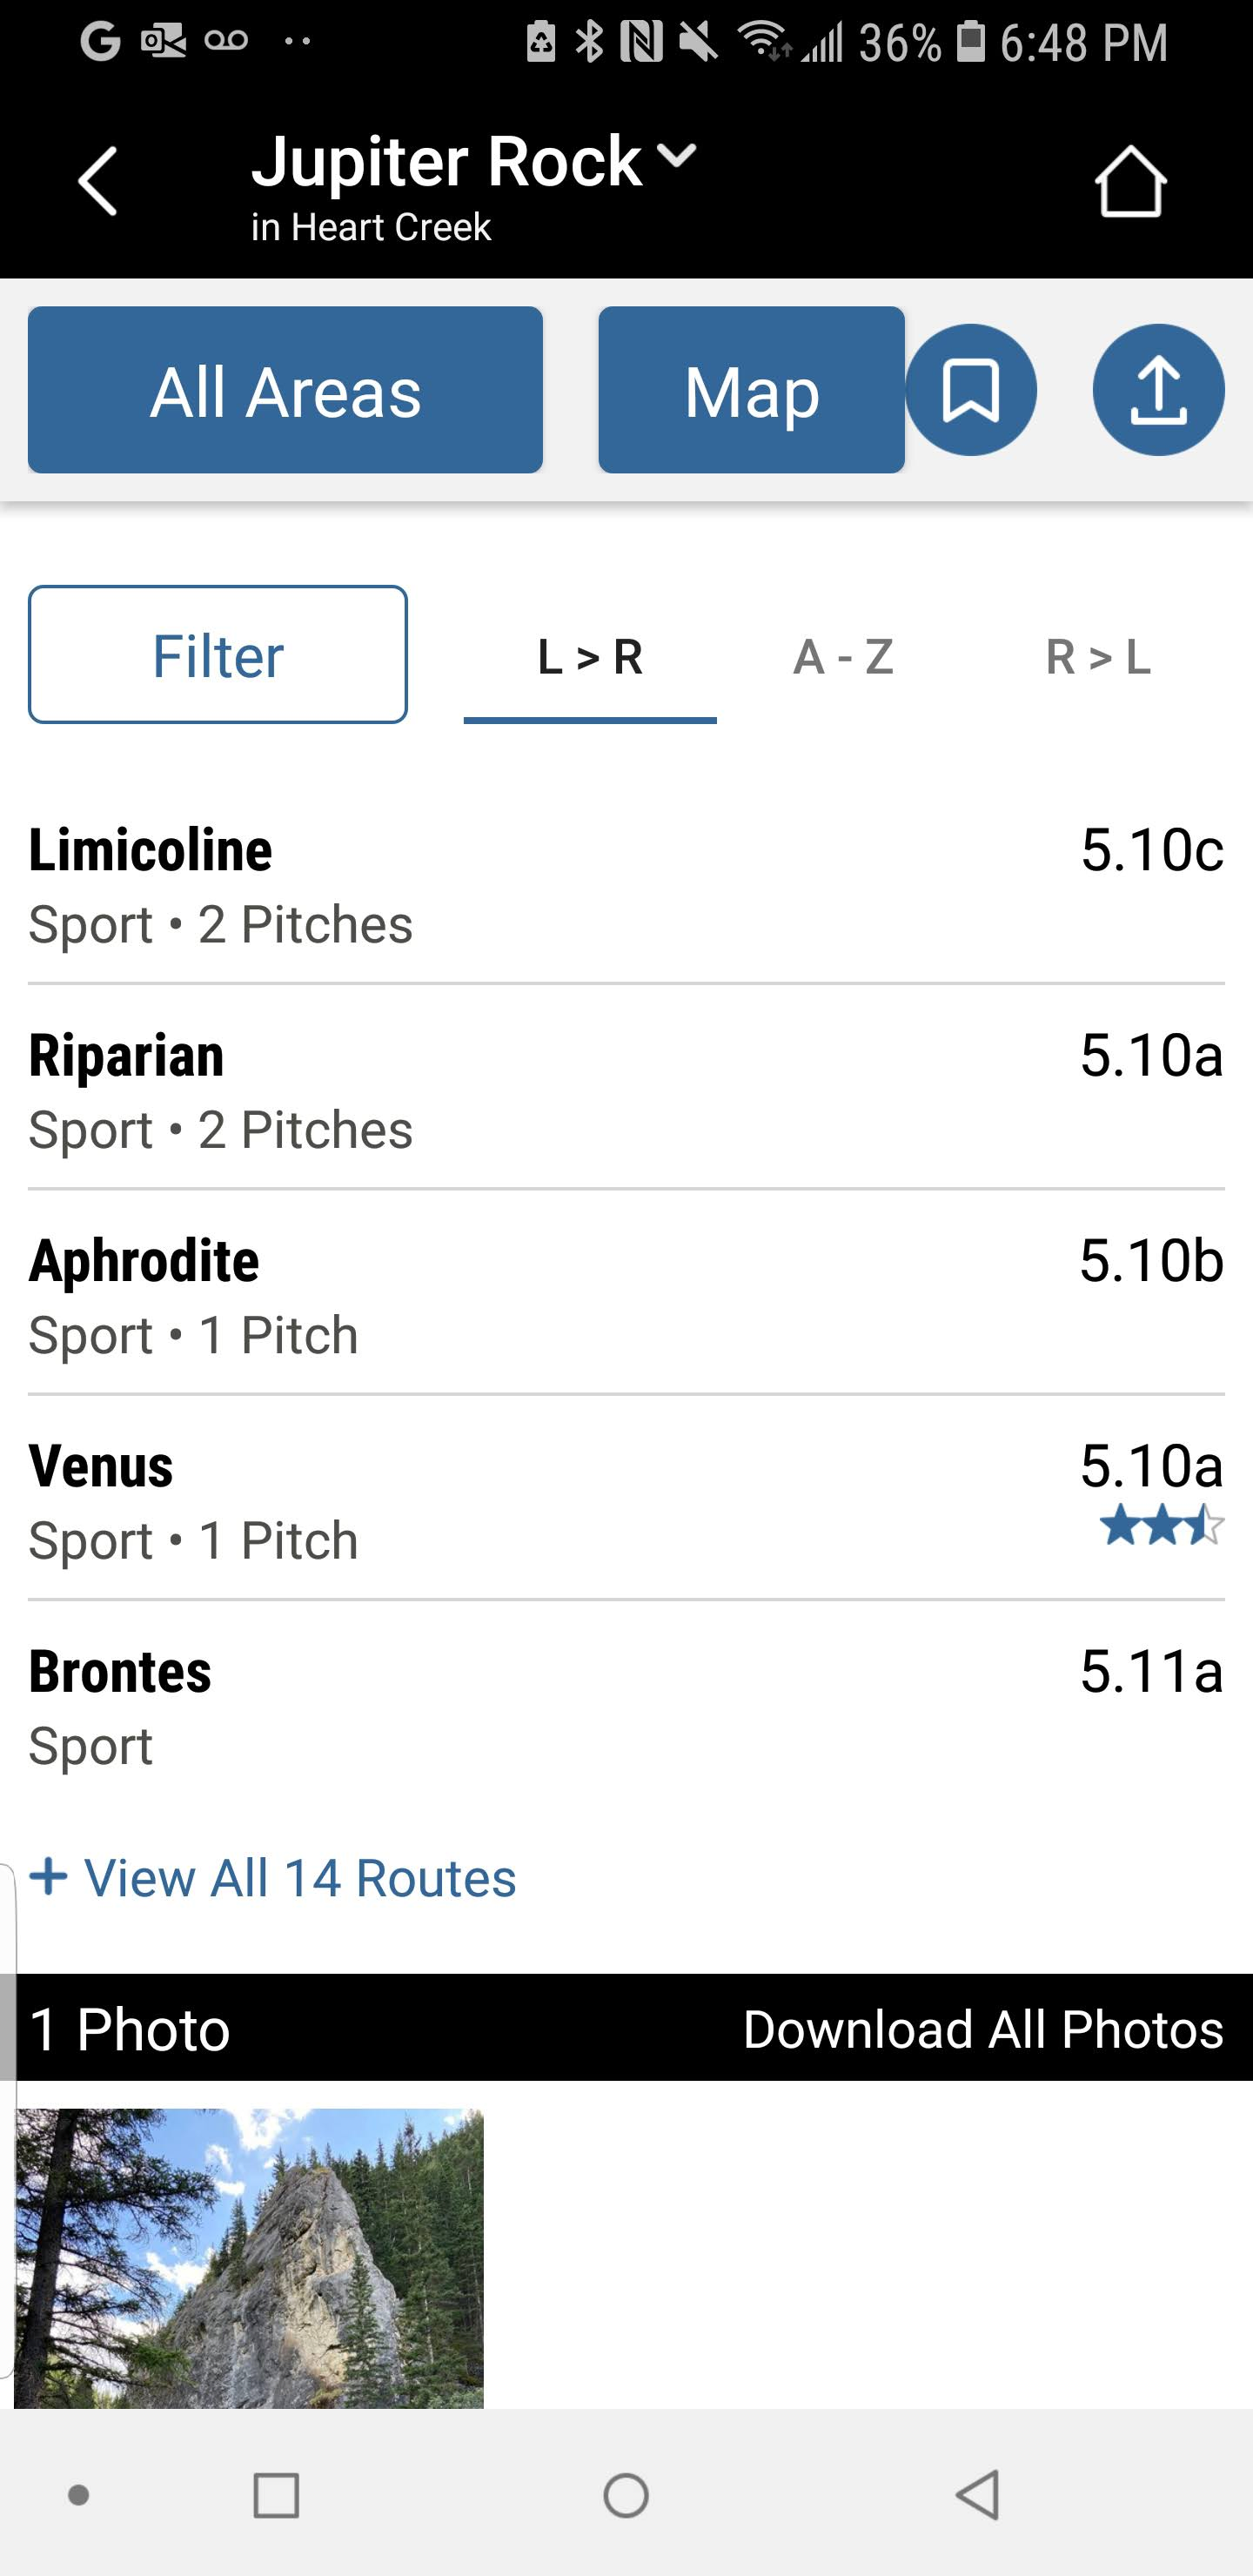
\includegraphics[width=\textwidth]{mp_jupiter_rock.jpg}
      \caption{Overview of specific rock face}
      \label{fig:face_overview}
  \end{subfigure}
  \caption{Route Selection UI interface for \emph{The Mountain Project}} 
\end{figure}

\begin{figure}[!h]
  \centering
  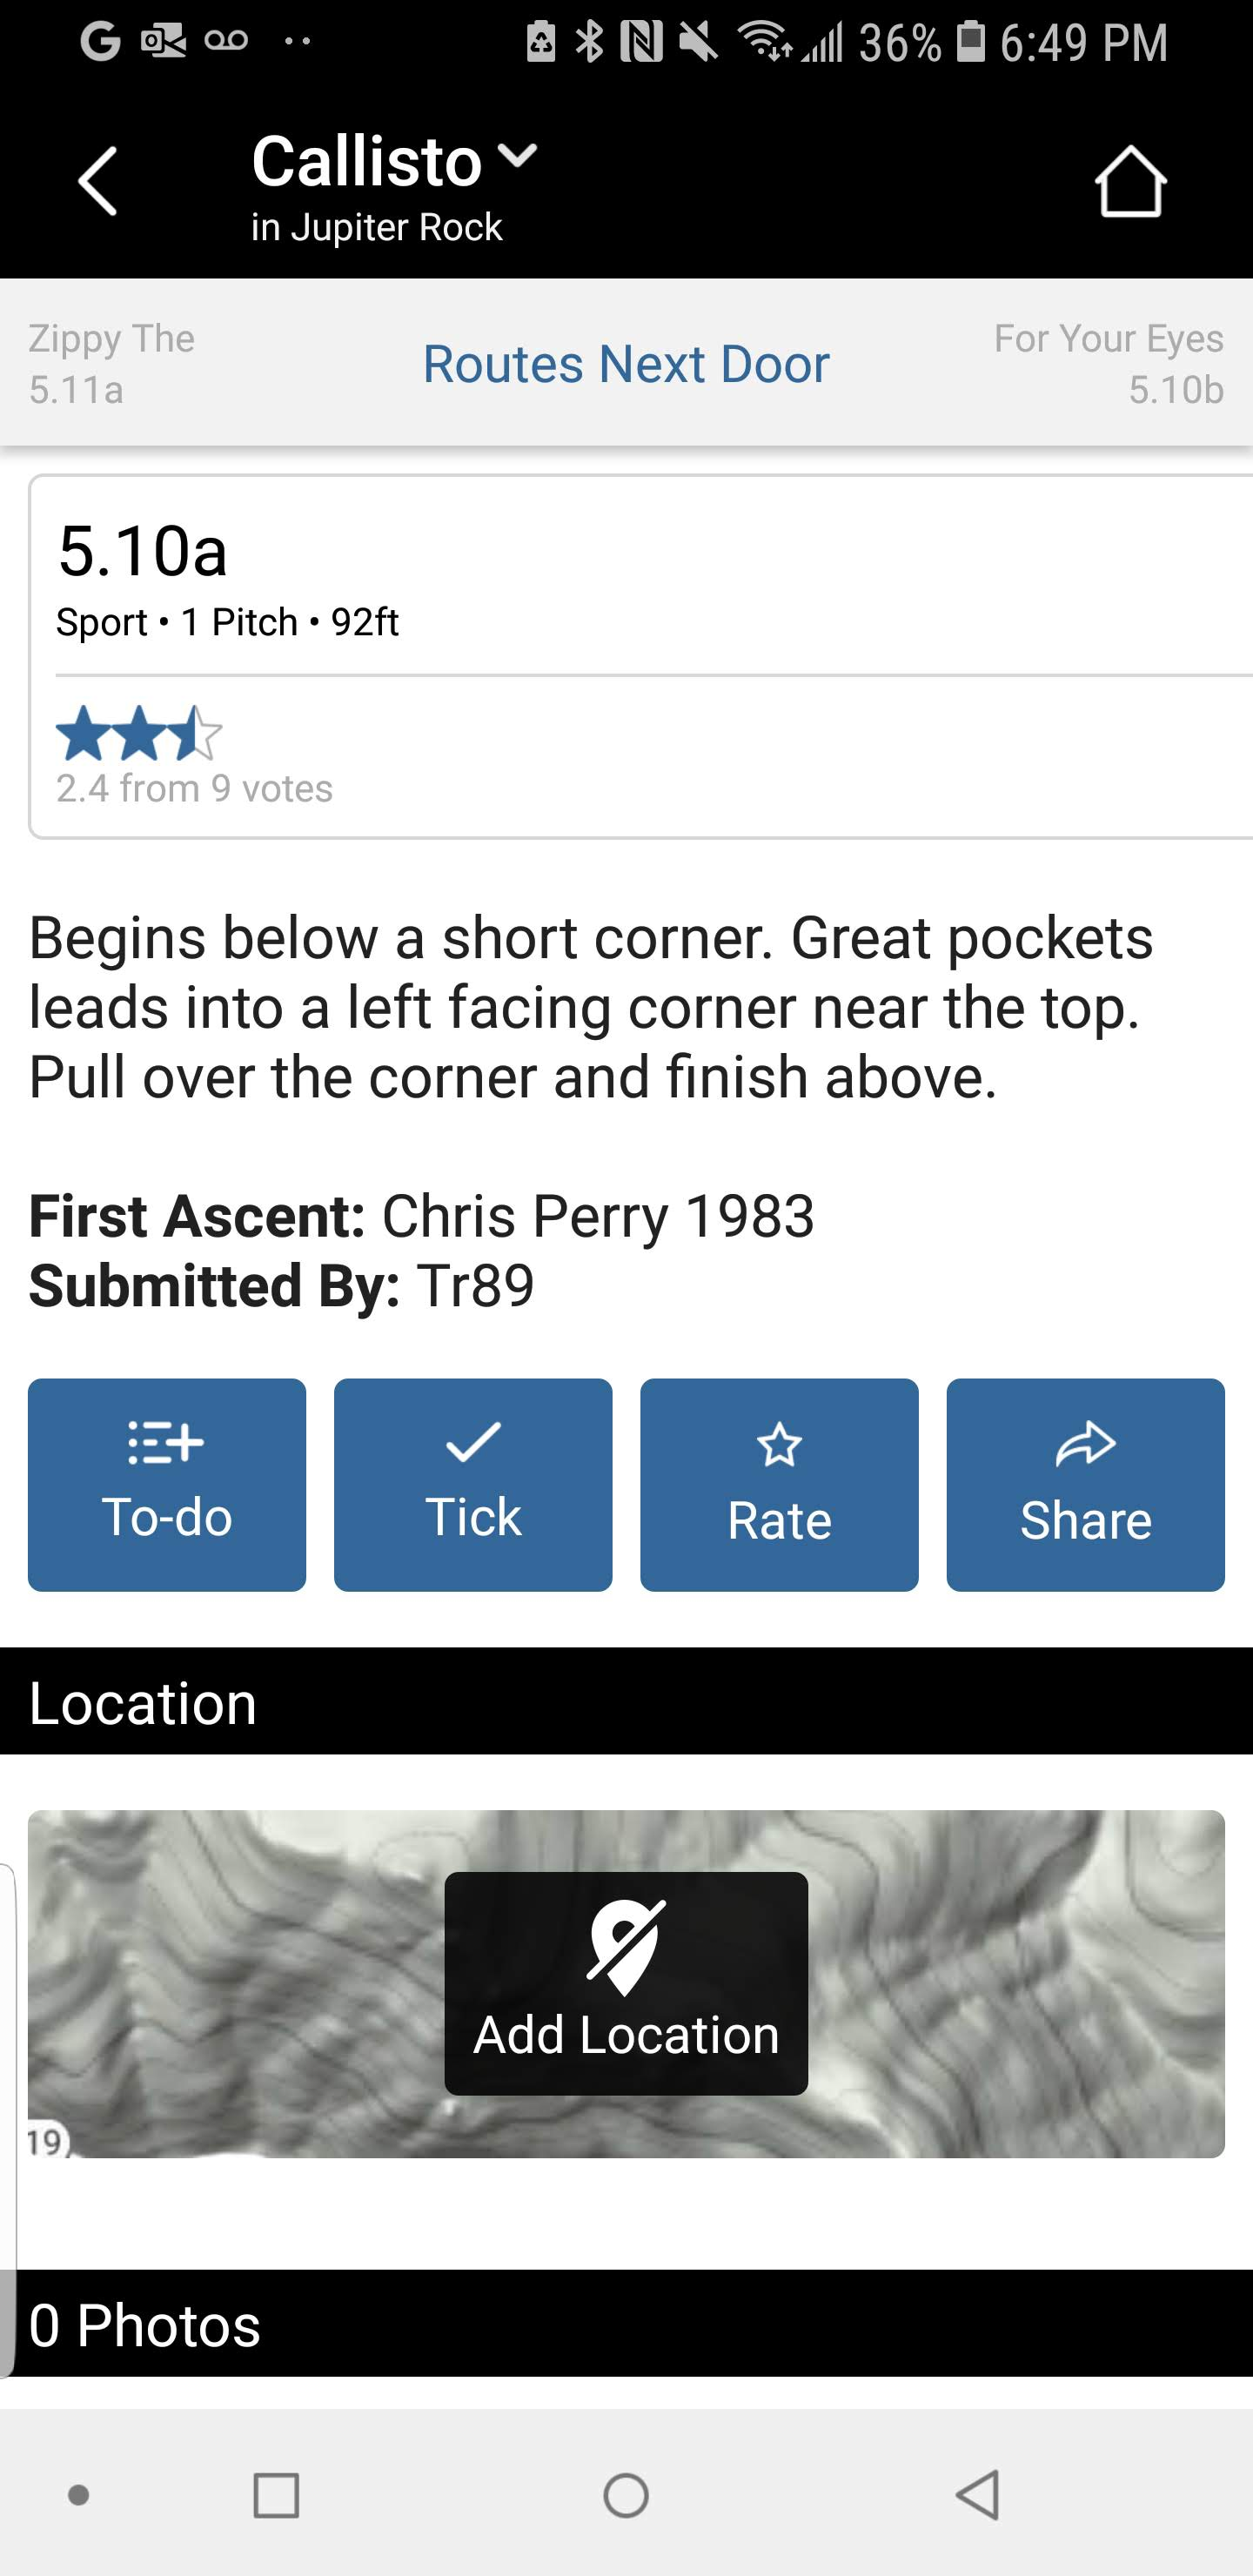
\includegraphics[width=0.25\textwidth]{mp_callisto.jpg}
  \caption{Route description page for Callisto}
  \label{fig:mp_callisto}
\end{figure}

\section{Conclusion}
All of the guidebooks were very similar in that the climbs were divided by region and plotted on either a photograph or drawing of the rock face. This suggests that users who are using the book in the field want to be able to correlate what they see in real life, with the route information in the book. The Mountain Project application contains many other features (such as search capabilities, route rating, an updatable to-do list) that are not really possible to implement in the form of a book. However, The Mountain Project is lacking as it does not have photographs with superimposed routes like the guidebooks do. It appears to be more of a search tool, than a visual aid for use in the field. The application we are designing could likely combine the best aspects of both the guidebooks (quickly identifying what routes are in front of the user) and The Mountain Project (advanced capabilities such as ratings, to-do list and search).

\pagebreak
\printbibliography

\end{document}